\documentclass[11pt,a4paper]{article}
\usepackage{fontspec}
\setmainfont{TeX Gyre Pagella}
\setsansfont{TeX Gyre Heros}
\usepackage[margin=21mm,top=24mm,bottom=23mm,headheight=15pt]{geometry}
\usepackage{amsmath,amssymb,graphicx,booktabs,tabularx,longtable,array,enumitem}
\usepackage[table]{xcolor}
\usepackage{tikz}
\usetikzlibrary{arrows.meta,positioning,calc,fit,backgrounds,shapes.geometric}
\usepackage[most]{tcolorbox}
\usepackage{fancyhdr,titlesec,hyperref,bookmark,microtype,needspace}
\definecolor{ink}{HTML}{172F3B}
\definecolor{teal}{HTML}{176C73}
\definecolor{rust}{HTML}{AA4F2D}
\definecolor{pale}{HTML}{EDF5F4}
\definecolor{warm}{HTML}{FCF2EB}
\definecolor{muted}{HTML}{576872}
\hypersetup{colorlinks=true,linkcolor=teal,urlcolor=teal,pdftitle={Power Systems Module 4 - Complete Study Notes},pdfauthor={Sudheesh},bookmarksdepth=2}
\urlstyle{same}
\setlength{\parindent}{0pt}
\setlength{\emergencystretch}{3em}
\setlength{\parskip}{4pt plus 1pt}
\setlist{itemsep=3pt,topsep=4pt,leftmargin=1.4em}
\renewcommand{\arraystretch}{1.22}
\newcolumntype{Y}{>{\raggedright\arraybackslash}X}
\newcolumntype{L}[1]{>{\raggedright\arraybackslash}p{#1}}
\pagestyle{fancy}\fancyhf{}
\fancyhead[L]{\footnotesize\sffamily\color{muted}POWER SYSTEMS / MODULE 4}
\fancyhead[R]{\footnotesize\sffamily\color{muted}PCEOT503}
\fancyfoot[L]{\footnotesize\sffamily\color{muted}Load flow and power system stability}
\fancyfoot[R]{\footnotesize\sffamily\thepage}
\renewcommand{\headrulewidth}{0.3pt}
\titleformat{\section}{\LARGE\sffamily\bfseries\color{ink}}{\thesection}{0.6em}{}
\titleformat{\subsection}{\large\sffamily\bfseries\color{teal}}{\thesubsection}{0.5em}{}
\titleformat{\subsubsection}{\normalsize\sffamily\bfseries\color{ink}}{}{0pt}{}
\titlespacing*{\section}{0pt}{12pt}{9pt}
\titlespacing*{\subsection}{0pt}{11pt}{5pt}
\titlespacing*{\subsubsection}{0pt}{8pt}{3pt}
\tcbset{enhanced,breakable,boxrule=0.4pt,arc=2pt,left=8pt,right=8pt,top=6pt,bottom=6pt,before skip=6pt,after skip=6pt,fonttitle=\sffamily\bfseries}
\newenvironment{Idea}[1]{\begin{tcolorbox}[colback=pale,colframe=teal,coltitle=white,title={#1}]}{\end{tcolorbox}}
\newenvironment{Caution}[1]{\begin{tcolorbox}[colback=warm,colframe=rust,coltitle=white,title={#1}]}{\end{tcolorbox}}
\newenvironment{Worked}[1]{\begin{tcolorbox}[breakable=false,colback=white,colframe=teal,colbacktitle=pale,coltitle=ink,title={#1}]}{\end{tcolorbox}}
\newcommand{\slides}[1]{{\small\color{muted}\textsf{Class-slide anchor: #1.}}\par}
\newcommand{\chapterstart}[2]{\par\needspace{12\baselineskip}\section{#1}\label{#2}}
\newcommand{\checkq}[2]{\begin{tcolorbox}[breakable=false,colback=pale,colframe=teal,coltitle=white,title={Check your understanding}]#1\par\textbf{Answer:} #2\end{tcolorbox}}
\tikzset{block/.style={draw=teal,fill=pale,rounded corners=2pt,align=center,text width=2.65cm,minimum height=1.0cm,font=\small\sffamily},hot/.style={block,draw=rust,fill=warm},arr/.style={-{Stealth[length=2.2mm]},thick,draw=ink},control/.style={arr,dashed,draw=rust}}
\newcommand{\diagramcaption}[1]{\par\smallskip{\small\color{muted}#1}\par}
\widowpenalty=10000\clubpenalty=10000
\newcommand{\ans}[1]{\boxed{#1}}
\newcommand{\phas}[2]{#1\angle #2^\circ}
\newcommand{\jj}{\mathrm j}
\begin{document}
\pagenumbering{roman}
\begin{titlepage}
\vspace*{12mm}
{\small\sffamily\color{teal}CET / SEMESTER 5 / PCEOT503}\par\vspace{16mm}
{\Huge\sffamily\bfseries\color{ink}POWER SYSTEMS}\par\vspace{6mm}
{\huge\sffamily\color{teal}Module 4}\par\vspace{10mm}
{\LARGE\sffamily Load flow and\\power system stability}\par\vspace{13mm}
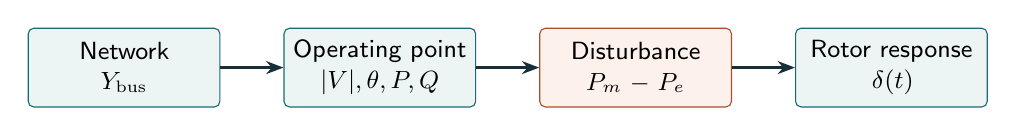
\begin{tikzpicture}[node distance=8mm]
\node[block,text width=2.2cm] (n) {Network\\$Y_{\rm bus}$};
\node[block,text width=2.2cm,right=of n] (v) {Operating point\\$|V|,\theta,P,Q$};
\node[hot,text width=2.2cm,right=of v] (d) {Disturbance\\$P_m-P_e$};
\node[block,text width=2.2cm,right=of d] (s) {Rotor response\\$\delta(t)$};
\draw[arr] (n)--(v);\draw[arr] (v)--(d);\draw[arr] (d)--(s);
\end{tikzpicture}\par\vspace{13mm}
\begin{Idea}{Two questions, one connected understanding}
What voltages and power flows exist at an operating point? After a disturbance, can the machines stay in synchronism? Learn the bus models, admittance matrix and Gauss--Seidel logic; then derive the power-angle curve, swing equation and equal-area criterion.
\end{Idea}
\vfill
{\small Comprehensive study notes covering load flow analysis and power system stability according to the 2024-scheme syllabus.}\par\vspace{4mm}
{\small\sffamily Prepared for Sudheesh / 8 October 2026}
\end{titlepage}
\setcounter{tocdepth}{1}\tableofcontents\clearpage\pagenumbering{arabic}

\chapterstart{Study map, scope and notation}{map}
\subsection{Every Module 4 syllabus requirement}
The supplied PCEOT503 syllabus assigns 11 contact hours to this module. Its two halves are steady-state network analysis and machine stability. A load-flow solution supplies an initial operating point for a stability study; it does not by itself prove that the system can survive a fault.
\begin{center}\small\begin{tabularx}{\textwidth}{L{.37\textwidth}Y}
\toprule Syllabus item & Developed in this note\\\midrule
Load-flow studies: introduction & Purpose, inputs, unknowns, outputs, operating checks, relation to fault/stability studies.\\
Types of buses & PQ, PV and slack; net injections, degrees of freedom, reactive limits and island references.\\
Network model and admittance matrix & Per-phase balanced model, line pi equivalent, KCL construction, properties, complete class three-bus example.\\
Gauss--Seidel: qualitative analysis & Update derivation, newest-value use, PQ/PV handling, flowchart, convergence, acceleration, merits/limits.\\
Steady-state, dynamic, transient stability & Definitions, physical distinctions, damping and disturbance size; limits of the classical model.\\
Power-angle curve; steady-state limit & SMIB circuit, derivation, stable/unstable equilibria, synchronizing coefficient and practical restrictions.\\
Swing equation & Torque-to-power derivation, mechanical/electrical angle conversion, inertia H, units, physical interpretation.\\
Equal-area criterion and application & Energy derivation, shaded areas, sudden input change, faults/clearing, line outage, clearing angle and time.\\
Improving stability limits & Electrical strength, fault-clearing speed, excitation/damping, mechanical-power control and operating margin.\\\bottomrule
\end{tabularx}\end{center}
\begin{Caution}{Respect the syllabus boundary on Gauss--Seidel}
The syllabus explicitly requires qualitative analysis and says numerical problems are not required. Learn the update equation and explain the flowchart. Section~\ref{classiteration} preserves the professor's one-iteration numerical illustration so no class material is lost, but it is labelled optional for exam preparation. The Y-bus example illustrates network construction; the stability examples explain the required derivations and applications.
\end{Caution}
\subsection{A learning sequence}
First understand what is specified at each bus. Derive Y-bus from KCL rather than memorizing its signs. Follow one qualitative Gauss--Seidel sweep and the PV correction. Next derive the sine power-angle curve; use its slope to understand restoring action. Derive the swing equation before studying shaded areas. Finally practise explaining why clearing the fault does not instantly stop the rotor-angle rise.

Sections~\ref{definitions}--\ref{improvements} develop power system stability, covering steady-state, dynamic, and transient stability analysis.
\subsection{Notation that prevents common mix-ups}
\begin{center}\small\begin{tabularx}{\textwidth}{L{.20\textwidth}Y}
\toprule Symbol & Meaning and convention\\\midrule
$V_i=v_i\angle\theta_i$ & Complex phase-voltage phasor at bus i; $v_i=|V_i|$. In per unit it uses the consistent three-phase system base.\\
$P_i,Q_i,S_i$ & Net bus injections into the network: $P_i=P_{Gi}-P_{Di}$, $Q_i=Q_{Gi}-Q_{Di}$, $S_i=P_i+\jj Q_i$.\\
$I_i$ & Net current injected into the network at bus i; $S_i=V_iI_i^*$ in consistent per unit.\\
$Y_{ij}=G_{ij}+\jj B_{ij}$ & Entry of the bus matrix. Lowercase $y_{ij}=1/z_{ij}$ denotes the series branch admittance; it is not the matrix off-diagonal.\\
$\theta_i$ versus $\delta$ & Bus angle versus generator internal-emf/rotor electrical angle relative to a synchronous reference. They need not be equal.\\
$P_m,P_e,P_a$ & Mechanical input, electrical output and accelerating power $P_a=P_m-P_e$. Losses are neglected in the basic swing equation.\\
$H,\omega_s$ & Stored kinetic energy at synchronous speed per MVA base, in seconds; electrical synchronous angular speed $\omega_s=2\pi f$.\\
$\delta_0,\delta_c,\delta_{\max},\delta_u$ & Initial, clearing, actual first-swing maximum and unstable post-fault equilibrium angles. The critical clearing angle is $\delta_{cr}$.\\\bottomrule
\end{tabularx}\end{center}
\begin{Idea}{Angles in equations}
Trigonometric sketches may label degrees. Differentiation, energy integration and clearing-time formulas use \textbf{electrical radians}. Convert degrees to radians before substituting. Subscripts ``max'' on $P_{\max}$ denote a curve height, whereas $\delta_{\max}$ is a trajectory's turning angle.
\end{Idea}

\chapterstart{What a load-flow study actually solves}{intro}
\slides{Load-flow deck, pp. 1--4, 19, 31}
\subsection{A bus is an electrical node}
A physical busbar connects generators, loads, lines and transformers at a substation. In a network model, components connected through ideal negligible-impedance links have the same bus voltage. A bus is therefore a node with one voltage magnitude and one phase angle in a balanced positive-sequence model.
\begin{center}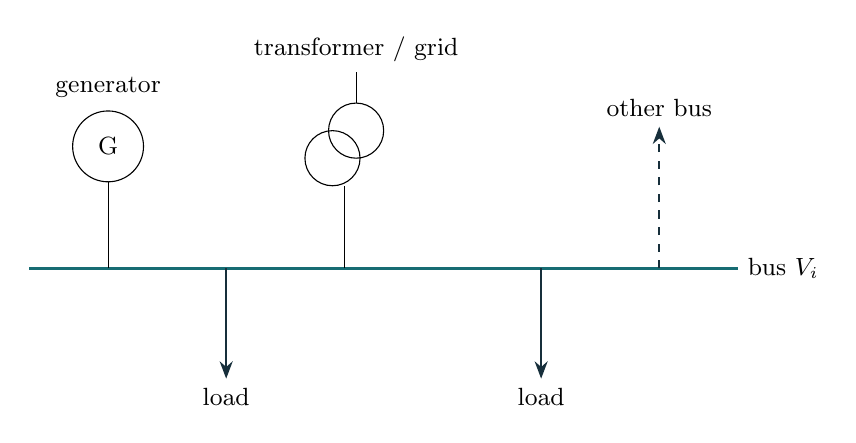
\begin{tikzpicture}[font=\small]
\draw[very thick,teal] (0,0)--(9,0);\node[right] at (9,0) {bus $V_i$};
\draw (1,0)--(1,1.1);\draw (1,1.55) circle(.45);\node at (1,1.55) {G};\node[above] at (1,2.05) {generator};
\draw (4,0)--(4,1.05);\draw (3.85,1.4) circle(.35);\draw (4.15,1.75) circle(.35);\draw (4.15,2.1)--(4.15,2.5);\node[above] at (4.15,2.5) {transformer / grid};
\draw[arr] (2.5,0)--(2.5,-1.4);\node[below] at (2.5,-1.4) {load};
\draw[arr] (6.5,0)--(6.5,-1.4);\node[below] at (6.5,-1.4) {load};
\draw[dashed,arr] (8,0)--(8,1.8);\node[above] at (8,1.8) {other bus};
\end{tikzpicture}\end{center}
\diagramcaption{Reconstruction of the image-only bus illustration on slide p. 4. Every connected element sees the same modeled bus voltage; its power contribution enters the net injection.}
\subsection{Why the study is needed}
A system can have enough installed generation and still have unacceptable bus voltages or overloaded lines. Power does not divide arbitrarily among paths: impedances and relative voltage phasors determine the division. A load-flow calculation finds a consistent set of phasors and flows for a particular pattern of generation, demand, network connections and controls.
\begin{itemize}
\item \textbf{Operation:} check voltage profile, generator reactive capability, line/transformer loading and losses before choosing an operating plan.
\item \textbf{Planning:} compare added lines, transformers, shunt compensation, generators and changed demand levels.
\item \textbf{Contingency assessment:} repeat the calculation after a selected outage to check whether the resulting steady state is feasible.
\item \textbf{Further analysis:} provide initial generator powers, terminal voltages and angles for a transient-stability study.
\end{itemize}
A conventional load flow is a steady-state algebraic calculation. It does not show the transient waveform after switching, the detailed short-circuit current, or the trajectory $\delta(t)$. Those require other models.
\subsection{What is input, and what is output?}
\begin{center}\small\begin{tabularx}{\textwidth}{Y Y}
\toprule Inputs & Outputs\\\midrule
Topology: buses, online branches and equipment connections. & Complex bus voltages, hence magnitudes and relative angles.\\
Line/transformer impedances, charging and shunts; taps as modeled. & Real/reactive power flow at both ends of every branch.\\
Loads, scheduled generator real powers, voltage setpoints and bus classifications. & Slack real/reactive injection and PV reactive requirements.\\
Common bases, generator Q limits, initial guesses and convergence tolerances. & Branch and total losses; voltages and loadings to compare against limits.\\\bottomrule
\end{tabularx}\end{center}
\begin{Caution}{Solving equations is different from enforcing limits}
A converged load flow can still violate a voltage limit, generator reactive limit or branch rating. The calculation supplies values to check; it does not automatically choose the least-cost generation or guarantee every limit. Optimal power flow is a different problem with objectives and constraints.
\end{Caution}
\subsection{Balanced per-unit modeling}
Use one common three-phase MVA base and voltage bases related by transformer ratios. Then $I_B=S_B/(\sqrt3V_{LL,B})$, $Z_B=V_{LL,B}^2/S_B$, $Y_B=1/Z_B$. In consistent per unit, the balanced three-phase relation is simply $S_i=V_iI_i^*$; an extra factor of three is not inserted. In physical units, per-phase power is $V_{ph}I_{ph}^*$ and total balanced power is three times that value.

Transmission load flow usually uses a balanced positive-sequence network. If phase unbalance is substantial, a three-phase formulation is required. Zero-sequence fault networks from Module 3 are not inserted into an ordinary balanced load-flow calculation.
\checkq{A study converges with all P/Q mismatches small. Is its operating point automatically acceptable?}{No. Compare its voltage magnitudes, generator Q outputs and branch currents/powers with their allowed ranges. Convergence proves equation consistency within tolerance, not operational acceptability.}

\chapterstart{PQ, PV and slack buses}{buses}
\slides{Load-flow deck, pp. 5--7, 19--20}
\subsection{Why only two of four quantities are specified}
At a bus, voltage has magnitude and angle, and power has real and reactive parts. These four numbers are linked by the network equations. For conventional bus classification, specify two and solve the other two. They are not four independently adjustable quantities.
\begin{center}\small\begin{tabularx}{\textwidth}{L{.15\textwidth}Y Y Y}
\toprule Bus & Specified & Solved & Typical interpretation\\\midrule
PQ / load & Net P and Q & $|V|$, angle & Demand modeled as constant power; also a generator at a binding Q limit.\\
PV / generator & Net P, $|V|$ & Net Q, angle & Generator adjusts reactive output to support its voltage setpoint within capability.\\
Slack / reference & $|V|$, angle & Net P, Q & Sets the angle reference and balances unscheduled injection/losses.\\\bottomrule
\end{tabularx}\end{center}
\begin{center}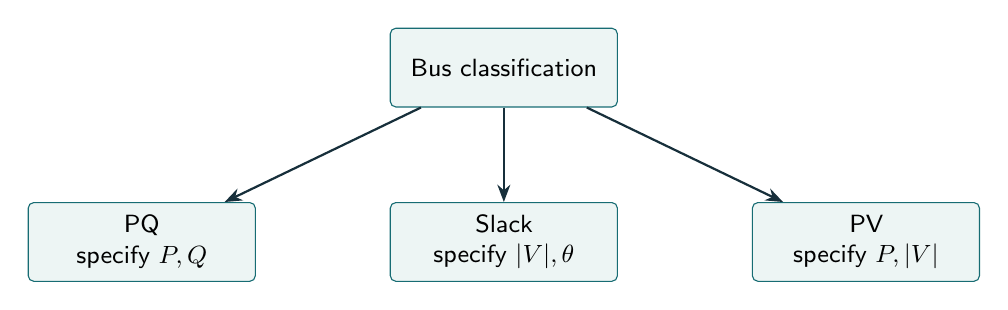
\begin{tikzpicture}[node distance=8mm]
\node[block] (b) {Bus classification};
\node[block,below left=12mm and 17mm of b] (q) {PQ\\specify $P,Q$};
\node[block,below=12mm of b] (s) {Slack\\specify $|V|,\theta$};
\node[block,below right=12mm and 17mm of b] (p) {PV\\specify $P,|V|$};
\draw[arr] (b)--(q);\draw[arr] (b)--(s);\draw[arr] (b)--(p);
\end{tikzpicture}\end{center}
\diagramcaption{The classification tree on image-only slide p. 5, reconstructed with the quantities each type fixes. A type describes a mathematical control condition, not merely the equipment name.}
\subsection{Net injection signs}
A load consumes power, so its network injection is negative. If a bus generates 80 MW and consumes 20 MW, its net real injection is 60 MW. If a generator bus also consumes 15 MVAr locally, the computed net reactive injection must be increased by 15 MVAr to obtain the generator reactive output.
\begin{Worked}{Sign and base example}
On a 100 MVA base, a bus has $P_G=80$ MW, $P_D=20$ MW, $Q_D=15$ MVAr and specified voltage 1.04 pu. Its scheduled $P_i=(80-20)/100=0.60$ pu. It is PV while voltage control is active. If the solution requires $Q_i=0.25$ pu, then $Q_G=25+15=40$ MVAr. Compare \emph{40 MVAr}, not 25 MVAr, with the generator limit.
\end{Worked}
\subsection{Why a slack is necessary}
Before solving, the line currents and hence real losses are unknown. If every generator's real output and every load's real demand were fixed independently, the chosen totals would generally not equal the eventual network losses. The conventional slack output is allowed to adjust so that the final solution balances.
\[
P_{G,slack}=\sum P_D+P_{loss}-\sum_{\text{other generators}}P_G.
\]
At its bus, the fixed voltage magnitude also leaves reactive injection free. The slack's Q is whatever the network solution demands at that voltage, subject to a later capability check.

Only angle differences affect the network powers. Adding the same angle to every voltage phasor changes no physical flow. Fixing one bus angle removes this redundant freedom. Zero degrees is convenient, not a special physical angle.
\begin{Caution}{One slack per connected island in the conventional formulation}
The slide's ``exactly one per power system'' statement assumes one connected network and the standard single-slack formulation. Separate energized islands need independent angle references and power balancing. Distributed-slack formulations can share the real-power adjustment among generators. The reference bus is not electrical earth: the voltage reference conductor and the phasor-angle reference play different roles.
\end{Caution}
The slack is a mathematical role; it need not be the largest generator in every study. A weak generator chosen as slack may end up with an infeasible output, so the resulting P and Q must be inspected. A negative slack P can be legitimate when other scheduled generation exceeds load and losses; it may also expose a scheduling/sign error.
\subsection{PV buses and reactive limits}
At a PV bus, Q is the adjustment needed to maintain voltage. A real generator cannot supply unlimited Q. If $Q_G$ exceeds $Q_{G,max}$ or falls below $Q_{G,min}$, fix it at the violated limit and use the corresponding net Q as a PQ specification. The voltage magnitude then becomes an unknown and may depart from its old setpoint.

The conceptual sequence is: estimate Q; recover generator Q including local demand; check capability; retain PV if feasible; otherwise clamp Q and solve as PQ. Detailed switching/re-entry rules vary by implementation; the syllabus requires understanding the physical reason, not a software-specific policy.
\checkq{Can a bus containing a generator be a PQ bus?}{Yes. A generator operated with fixed P and Q, or a voltage-controlling generator that has reached a reactive limit, can be modeled as PQ. The bus type reflects which quantities are controlled.}
\subsection{Counting unknowns}
For $n_{PQ}$ load buses, $n_{PV}$ voltage-controlled buses and one conventional slack, the unknown voltage quantities are $2n_{PQ}+n_{PV}$: magnitudes/angles at PQ buses and angles at PV buses. Solve real-power balance at every non-slack bus and reactive-power balance at each PQ bus. PV Q and slack P/Q are then obtained from the solved voltages.

\chapterstart{Network model and the bus admittance matrix}{ybus}
\slides{Load-flow deck, pp. 8--16}
\subsection{A branch joins two voltage nodes}
A short-line approximation uses a series impedance $z_{ij}=r_{ij}+\jj x_{ij}$. A nominal-pi representation also puts half the line's total shunt charging admittance at each end. Shunt reactors and capacitors at a bus are additional connections to the reference conductor. The series and shunt parts have different matrix contributions.
\begin{center}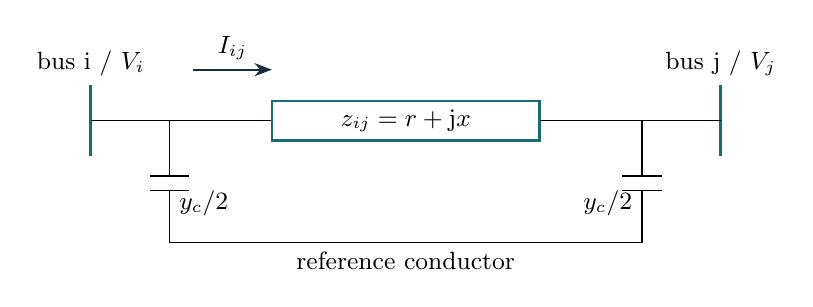
\begin{tikzpicture}[font=\small]
\draw[very thick,teal] (0,-.45)--(0,.45);\draw[very thick,teal] (8,-.45)--(8,.45);
\draw (0,0)--(2.3,0);\draw[teal,thick] (2.3,-.25) rectangle (5.7,.25);\node at (4,0) {$z_{ij}=r+\jj x$};\draw (5.7,0)--(8,0);
\node[above] at (0,.45) {bus i / $V_i$};\node[above] at (8,.45) {bus j / $V_j$};
\foreach \x in {1,7}{\draw (\x,0)--(\x,-.7);\draw (\x-.25,-.7)--(\x+.25,-.7);\draw (\x-.25,-.88)--(\x+.25,-.88);\draw (\x,-.88)--(\x,-1.55);}
\draw (1,-1.55)--(7,-1.55);\node[below] at (4,-1.55) {reference conductor};\node[right] at (1,-1.05) {$y_c/2$};\node[left] at (7,-1.05) {$y_c/2$};
\draw[arr] (1.3,.65)--(2.3,.65);\node[above] at (1.8,.65) {$I_{ij}$};
\end{tikzpicture}\end{center}
\subsection{Derive a row from Kirchhoff's current law}
For an ordinary untapped branch, current leaving bus i towards j is $y_{ij}(V_i-V_j)$, where $y_{ij}=1/z_{ij}$. Let $y_{sh,i}$ include all modeled shunts at bus i, including line-end charging terms. Net injection equals the sum of currents leaving into those elements:
\begin{align*}
I_i&=\sum_{j\ne i}y_{ij}(V_i-V_j)+y_{sh,i}V_i\\
&=\left(\sum_{j\ne i}y_{ij}+y_{sh,i}\right)V_i-\sum_{j\ne i}y_{ij}V_j.
\end{align*}
Therefore, for the ordinary branch model,
\[
\boxed{Y_{ii}=\sum_{j\ne i}y_{ij}+y_{sh,i}},\qquad
\boxed{Y_{ij}=-y_{ij}\quad(i\ne j)}.
\]
If several parallel branches join i and j, add their admittances before applying the minus sign. If no branch couples the pair, that off-diagonal is zero. This construction gives the compact linear current-voltage relation
\[
\boxed{\mathbf I=Y_{\rm bus}\mathbf V}.
\]
\begin{Idea}{An easy physical check on the minus sign}
If $V_i=V_j$ and there are no shunts, the branch current must be zero. The row contribution $yV_i-yV_j$ gives exactly that. A positive off-diagonal equal to $+y$ would not.
\end{Idea}
\subsection{Assembly as a branch stamp}
For an ordinary branch $y$ joining i and j, add the following into the matrix at the corresponding rows and columns:
\[
\begin{bmatrix}\Delta Y_{ii}&\Delta Y_{ij}\\\Delta Y_{ji}&\Delta Y_{jj}\end{bmatrix}
=\begin{bmatrix}y&-y\\-y&y\end{bmatrix}.
\]
Add each shunt only to its bus's diagonal. Assemble contributions branch by branch. This is often less error-prone than drawing an entire matrix at once.
\subsection{What properties are safe to claim?}
\begin{itemize}
\item \textbf{Complex:} resistance/conductance and reactance/susceptance are both allowed. The matrix is not generally real or Hermitian.
\item \textbf{Sparse:} a bus connects directly to relatively few others, so most off-diagonals of a large ordinary network are zero.
\item \textbf{Symmetric under the basic reciprocal model:} untapped lines and ordinary real-ratio tap models give $Y_{ij}=Y_{ji}$. A phase-shifting transformer can make these different. Passivity alone is not the sufficient blanket condition asserted by the slide.
\item \textbf{Row sums:} for ordinary untapped branches they equal the connected shunt admittance. With no shunts, each row sum is zero. This property changes with off-nominal transformer taps.
\item \textbf{Diagonal magnitude:} it is often large in a simple inductive network, but it is not universally the largest entry. Capacitive and inductive admittances can cancel.
\end{itemize}
With no shunts, $Y\mathbf1=0$ for the untapped connected network, so the unreduced Y-bus is singular. This does not prevent load flow: the specified slack phasor supplies the missing reference/boundary condition, and the nonlinear power equations are solved for the remaining voltages.
\subsection{Optional transformer model: why exceptions occur}
A real transformer leakage branch can have an off-nominal complex tap $a=\tau e^{\jj\phi}$ at the i end. A standard pi branch stamp is
\[
\begin{bmatrix}
(y+\jj b_c/2)/|a|^2 & -y/a^*\\
-y/a & y+\jj b_c/2
\end{bmatrix}.
\]
For a phase shift $\phi\ne0$, off-diagonals are generally unequal. This is explanatory context beyond the slides' simple three-bus example; ordinary untapped KCL construction is the principal syllabus model. A transformer phase shift is a modeled electrical relation, not the arbitrary common phasor reference.
\checkq{An inductive line has $z=\jj0.1$ pu. What are its series admittance and ordinary off-diagonal matrix contribution?}{$y=1/(\jj0.1)=-\jj10$ pu. The matrix off-diagonal is $-y=+\jj10$ pu. Mixing up y with Y reverses the sign.}

\chapterstart{Complete class Y-bus example}{classexample}
\slides{Load-flow deck, pp. 12--16; reused on p. 23}
The class network has three buses and three inductive series branches, with no line charging or bus shunts:
\[
z_{12}=\jj0.10,\quad z_{13}=\jj0.20,\quad z_{23}=\jj0.25\quad\text{pu}.
\]
\begin{center}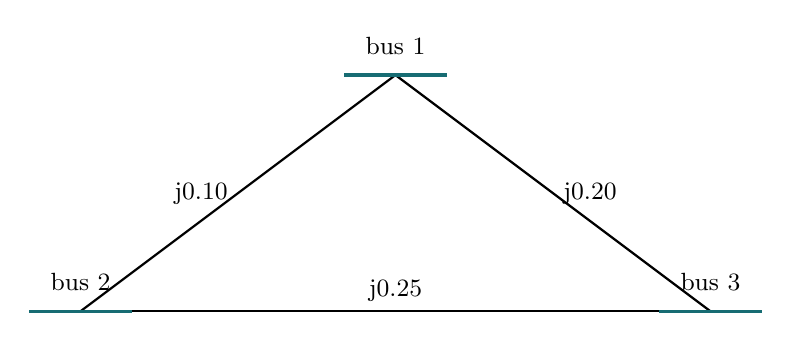
\begin{tikzpicture}[font=\small]
\coordinate (a) at (4,3);\coordinate (b) at (0,0);\coordinate (c) at (8,0);
\draw[thick] (a)--node[left] {$\jj0.10$} (b);\draw[thick] (a)--node[right] {$\jj0.20$} (c);\draw[thick] (b)--node[above] {$\jj0.25$} (c);
\foreach \p/\l in {a/1,b/2,c/3}{\draw[teal,very thick] ($(\p)+(-.65,0)$)--($(\p)+(.65,0)$);\node[above=4pt] at (\p) {bus \l};}
\end{tikzpicture}\end{center}
\diagramcaption{All branch values are on one common base. This reconstructs the original network diagrams on pp. 12 and 23; p. 16's image-only final matrix is developed explicitly below.}
\subsection{Step 1: reciprocal each impedance}
\[
y_{12}=-\jj10,\qquad y_{13}=-\jj5,\qquad y_{23}=-\jj4.
\]
The inverse of $\jj x$ is $-\jj/x$, not $+\jj/x$.
\subsection{Step 2: sum admittances at each bus}
\begin{align*}
Y_{11}&=y_{12}+y_{13}=-\jj15,\\
Y_{22}&=y_{12}+y_{23}=-\jj14,\\
Y_{33}&=y_{13}+y_{23}=-\jj9.
\end{align*}
\subsection{Step 3: negate the mutual branch admittances}
\[
Y_{12}=Y_{21}=+\jj10,\quad Y_{13}=Y_{31}=+\jj5,\quad
Y_{23}=Y_{32}=+\jj4.
\]
\subsection{Step 4: assemble and check}
\[
\boxed{Y_{\rm bus}=\begin{bmatrix}
-\jj15&\jj10&\jj5\\
\jj10&-\jj14&\jj4\\
\jj5&\jj4&-\jj9
\end{bmatrix}\ \text{pu}}.
\]
It is symmetric. Each row sums to zero because the example has only ordinary series branches and no shunts. For $V_1=V_2=V_3$, all branch currents vanish, consistent with this check. No bus load is added to this matrix as a fixed admittance when that load is already specified as constant P and Q.
\begin{Worked}{An original small modification}
Add a capacitive shunt $y_{sh,2}=\jj0.20$ pu at bus 2. Only $Y_{22}$ changes: $-\jj14+\jj0.20=-\jj13.80$. The second row now sums to $\jj0.20$, while the other rows still sum to zero. At a given voltage, the shunt supplies reactive power; its modeled admittance belongs in the network once, not again as a duplicate Q injection.
\end{Worked}
\subsection{A physical KCL row}
At bus 2, with no shunt,
\[
I_2=-\jj10(V_2-V_1)-\jj4(V_2-V_3)
=\jj10V_1-\jj14V_2+\jj4V_3.
\]
This is exactly row 2 of the matrix. If an answer has a different row, return to this simple current balance and find which branch or sign was misplaced.

\chapterstart{From current equations to power equations}{powereq}
\slides{Load-flow deck, pp. 18--21}
\subsection{Why a linear network gives a nonlinear load flow}
For fixed branch parameters, $I=YV$ is linear. But the specified bus quantities are powers, and complex power multiplies voltage by the conjugate of current:
\[
S_i=P_i+\jj Q_i=V_iI_i^*
=V_i\left(\sum_jY_{ij}V_j\right)^*.
\]
Equivalently,
\[
\boxed{P_i-\jj Q_i=V_i^*\sum_jY_{ij}V_j}.
\]
The product of voltage variables and the voltage in the power-to-current conversion create the nonlinearity. A PQ load's current changes as its voltage changes; it is not a fixed injection throughout iteration.
\begin{Idea}{What the denominator means}
From $S_i^*=V_i^*I_i$, the specified-power injection current is $I_i=(P_i-\jj Q_i)/V_i^*$. If voltage is lower, a constant-power load draws a larger current magnitude. This feedback helps explain difficulty near heavily loaded operating points.
\end{Idea}
\subsection{Polar real and reactive equations}
Writing $Y_{ij}=G_{ij}+\jj B_{ij}$ and $V_i=v_ie^{\jj\theta_i}$ gives
\begin{align*}
P_i&=v_i\sum_jv_j\left[G_{ij}\cos(\theta_i-\theta_j)+B_{ij}\sin(\theta_i-\theta_j)\right],\\
Q_i&=v_i\sum_jv_j\left[G_{ij}\sin(\theta_i-\theta_j)-B_{ij}\cos(\theta_i-\theta_j)\right].
\end{align*}
These equations display the coupling between voltage magnitudes and angles. They also explain why ``P controls angle and Q controls voltage'' is an approximation that is useful in many high-X/R transmission networks, rather than an exact universal separation.
\subsection{Specify only the proper equations}
At a PQ bus, match both P and Q. At a PV bus, match P while enforcing its voltage magnitude; compute its Q. At the slack, keep the voltage phasor fixed and compute P/Q afterwards. This keeps the problem neither under- nor over-specified.

The diagram-like equations on image-only slide p. 21 are recovered by rearranging one KCL row:
\[
Y_{ii}V_i=I_i-\sum_{j\ne i}Y_{ij}V_j,
\qquad
\boxed{V_i=\frac1{Y_{ii}}\left[\frac{P_i-\jj Q_i}{V_i^*}-\sum_{j\ne i}Y_{ij}V_j\right]}.
\]
This is an implicit identity: $V_i$ appears on both sides. Gauss--Seidel uses the current estimate in the denominator and the most recently available neighbouring voltages to obtain the next estimate.
\checkq{Why not simply calculate $V=Y^{-1}I$ once?}{The specified inputs are generally powers, not fixed currents. At constant P/Q, $I_i=S_i^*/V_i^*$ changes with the unknown voltage. Also the unreduced no-shunt Y-bus can be singular. A reference and nonlinear solution are needed.}

\chapterstart{Gauss--Seidel load flow: the qualitative method}{gs}
\slides{Load-flow deck, pp. 17--22, 28--30}
\subsection{The defining idea: use each new answer immediately}
Choose starting estimates for unknown voltage phasors. Visit buses in an order. Update one bus using its specified power and the current estimates at the others; use that new voltage when visiting the next bus in the same sweep. Repeat sweeps until the specified equations are adequately satisfied.

In a Jacobi-style simultaneous update, all buses would use the previous sweep's voltages. Gauss--Seidel's immediate reuse is the distinction to explain in an exam. It does not mean bus 3's physical voltage waits for bus 2; the order belongs to the numerical algorithm.
\subsection{PQ update equation and every term}
Take bus 1 as slack and let k denote the completed sweep count. For a non-slack PQ bus i,
\[
\boxed{V_i^{(k+1)}=\frac{1}{Y_{ii}}\left[
\frac{P_i-\jj Q_i}{(V_i^{(k)})^*}
-\sum_{j<i}Y_{ij}V_j^{(k+1)}
-\sum_{j>i}Y_{ij}V_j^{(k)}\right]}.
\]
\begin{itemize}
\item $P_i,Q_i$ are scheduled \emph{net} injections; load-only buses normally have negative values.
\item The denominator is the conjugate of the bus's voltage estimate. Omitting the conjugate changes the equation.
\item The first sum uses voltages already updated in this sweep; the second uses voltages not yet updated.
\item The slack phasor is the same in every sweep. It is used whenever its term appears; it is never updated by this PQ formula.
\item $Y_{ii}$ is the self-admittance from the actual network, including modeled shunts/taps, not an individual branch admittance.
\end{itemize}
\subsection{Initialization}
A flat start puts unknown PQ phasors at $1\angle0^\circ$ pu. Start PV magnitudes at their specified setpoints, normally with zero initial angle, and keep the specified slack phasor. A previous solved operating point may give a better initial estimate for a nearby study. An initial guess is not an extra specified physical voltage.
\subsection{PV update, without pretending Q is known}
At the current estimates, calculate the net reactive injection from
\[
\boxed{Q_i=-\operatorname{Im}\left\{V_i^*\sum_jY_{ij}V_j\right\}}.
\]
Compute required generator Q including local demand and check its limits. If the bus remains PV, put the estimated Q in the voltage update to obtain a temporary complex $\widetilde V_i$. Retain its angle but restore the specified magnitude:
\[
\boxed{V_i^{new}=v_i^{spec}\frac{\widetilde V_i}{|\widetilde V_i|}}.
\]
It is a radial projection in the complex-voltage plane. It does not set the angle to zero. If Q has been clamped at a limit, treat the bus as PQ and do not simultaneously enforce its former PV magnitude.
\begin{center}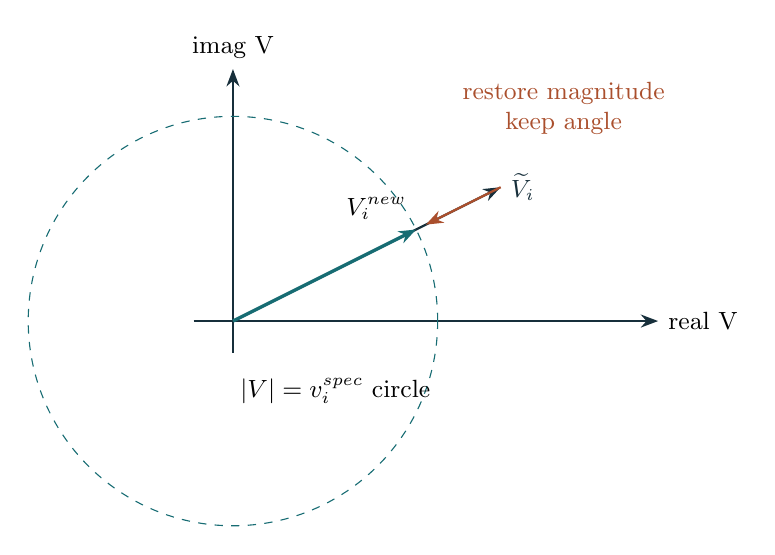
\begin{tikzpicture}[font=\small]
\draw[arr] (-.5,0)--(5.4,0) node[right] {real V};\draw[arr] (0,-.4)--(0,3.2) node[above] {imag V};
\draw[teal,dashed] (0,0) circle(2.6);\draw[arr,ink] (0,0)--(3.4,1.7) node[right] {$\widetilde V_i$};
\draw[arr,teal,very thick] (0,0)--(2.3255,1.1628);\node[above left] at (2.3255,1.1628) {$V_i^{new}$};
\draw[arr,rust] (3.4,1.7)--(2.45,1.225);\node[rust,align=center] at (4.2,2.7) {restore magnitude\\keep angle};\node[below] at (1.3,-.6) {$|V|=v_i^{spec}$ circle};
\end{tikzpicture}\end{center}
\diagramcaption{A conceptual PV projection. The orientation is illustrative; a generator angle can be positive or negative depending on the chosen reference and operating point.}
\subsection{A complete qualitative flowchart}
\begin{center}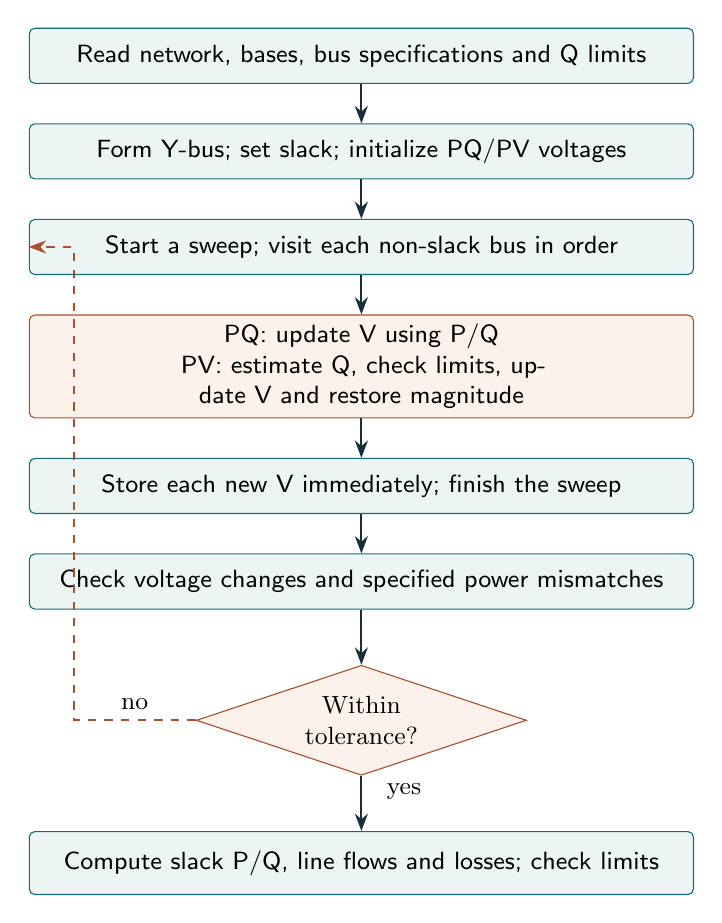
\begin{tikzpicture}[node distance=5mm, font=\small]
\node[block,text width=8.2cm,minimum height=.7cm] (a) {Read network, bases, bus specifications and Q limits};
\node[block,text width=8.2cm,minimum height=.7cm,below=of a] (b) {Form Y-bus; set slack; initialize PQ/PV voltages};
\node[block,text width=8.2cm,minimum height=.7cm,below=of b] (c) {Start a sweep; visit each non-slack bus in order};
\node[hot,text width=8.2cm,minimum height=.9cm,below=of c] (d) {PQ: update V using P/Q\\PV: estimate Q, check limits, update V and restore magnitude};
\node[block,text width=8.2cm,minimum height=.7cm,below=of d] (e) {Store each new V immediately; finish the sweep};
\node[block,text width=8.2cm,minimum height=.7cm,below=of e] (f) {Check voltage changes and specified power mismatches};
\node[draw=rust,fill=warm,diamond,aspect=3,align=center,below=7mm of f] (g) {Within\\tolerance?};
\node[block,text width=8.2cm,minimum height=.8cm,below=7mm of g] (h) {Compute slack P/Q, line flows and losses; check limits};
\foreach \x/\y in {a/b,b/c,c/d,d/e,e/f,f/g,g/h}{\draw[arr] (\x)--(\y);}
\node[right] at ($(g.south)+(.2,-.2)$) {yes};
\draw[control] (g.west)--node[above] {no} ++(-1.55,0)|-(c.west);
\end{tikzpicture}\end{center}
Set an iteration limit so an unsuccessful solve is reported rather than looping forever. A failed solve calls for checking inputs, controls, guesses and feasibility; it is not by itself proof that the physical system has already lost synchronism.
\subsection{Convergence: what does ``small enough'' mean?}
The slides use a voltage-change test such as $\max_i|V_i^{new}-V_i^{old}|<\varepsilon_V$. A value such as $10^{-4}$ pu is an illustrative tolerance. A stronger check computes the residuals of the specified power equations:
\[
\Delta P_i=P_i^{spec}-P_i^{calc},\qquad
\Delta Q_i=Q_i^{spec}-Q_i^{calc}.
\]
Check $\Delta P$ at all non-slack buses and $\Delta Q$ at PQ buses. PV buses instead have a magnitude constraint. Small voltage steps can occur during slow progress or poor scaling while a power mismatch remains material; inspect the mismatches too.
\subsection{Acceleration factor}
An extrapolated update is
\[
V_i^{acc}=V_i^{old}+\alpha(\widetilde V_i-V_i^{old}).
\]
Here $\widetilde V_i$ is the calculated unaccelerated update. $\alpha=1$ is ordinary Gauss--Seidel. A suitable value above one can reduce iterations; a value below one damps updates and can help in difficult cases. The slides' 1.4--1.6 range is a common example, not a guaranteed optimum for every nonlinear power system. Aggressive overcorrection can diverge. Classical convergence rules for linear systems must not be treated as universal nonlinear load-flow guarantees.

For a bus remaining PV, enforce its specified magnitude after the chosen complex correction. There is no reason to accelerate the fixed slack. Algorithm details should be stated consistently when comparing iteration counts.
\subsection{Merits, limits and the other methods in the slides}
Gauss--Seidel is conceptually transparent, simple to implement, and needs modest storage for a small sparse network. Its iteration count can be high; sensitivity to starting guess, bus order, loading, controls and network conditioning makes it less attractive for large difficult systems. Series compensation/negative branch reactance can complicate convergence, but it does not universally prevent a solution.
\begin{center}\small\begin{tabularx}{\textwidth}{L{.23\textwidth}Y Y}
\toprule Method & Main idea & Useful qualification\\\midrule
Gauss--Seidel & Sequential voltage substitutions, newest values reused. & Simple; may converge slowly or fail from an unsuitable guess/model.\\
Newton--Raphson & Solve mismatch corrections using a Jacobian. & Fast local convergence near a regular solution; not globally guaranteed.\\
Fast decoupled & Approximate the P-angle and Q-voltage coupling. & Efficient under suitable transmission-system assumptions; accuracy/convergence suffer when assumptions are weak.\\\bottomrule
\end{tabularx}\end{center}
Newton--Raphson and fast-decoupled methods appear on slide p. 30 as context. Their detailed derivations are not additional requirements of this syllabus. Multiple mathematical power-flow solutions can exist. Finding one solution does not establish its operating suitability, and a low-voltage branch is a reason for examination, not an automatic universal stability diagnosis.
\checkq{Explain a PV bus in one sentence within a Gauss--Seidel sweep.}{Estimate its reactive injection, check generator Q capability, perform a complex voltage update, and restore the prescribed magnitude while retaining the new angle if voltage control remains feasible.}

\chapterstart{The professor's one-iteration illustration}{classiteration}
\slides{Load-flow slides pp. 23--27. Optional numerical illustration: Gauss--Seidel numerical problems are not required by this syllabus.}
\subsection{Data and the signs that matter}
Use the same lossless three-bus network as Section~\ref{classexample}. The slack voltage is $V_1=1+\jj0$. The loads are $0.5+\jj0.2$ pu at bus 2 and $0.4+\jj0.3$ pu at bus 3. Therefore the \emph{net injections} used in the equations are
\[
S_2=-0.5-\jj0.2,\qquad S_3=-0.4-\jj0.3.
\]
The flat start is $V_2^{(0)}=V_3^{(0)}=1$. Use ordinary Gauss--Seidel with $\alpha=1$. We calculate bus 2 before bus 3.
\subsection{Update bus 2}
Since $P_2-\jj Q_2=-0.5+\jj0.2$, the first substitution is
\begin{align*}
V_2^{(1)}&=\frac{1}{-\jj14}\left[\frac{-0.5+\jj0.2}{1}-\jj10(1)-\jj4(1)\right]\\
&=\frac{-0.5-\jj13.8}{-\jj14}
=\ans{0.985714-\jj0.035714}\ \mathrm{pu}.
\end{align*}
Its magnitude and angle are $0.986361$ pu and $-2.0750^\circ$. The change is $|V_2^{(1)}-1|=0.038465$ pu.
\subsection{Update bus 3 using the NEW bus-2 voltage}
\begin{align*}
V_3^{(1)}&=\frac{1}{-\jj9}\left[\frac{-0.4+\jj0.3}{1}-\jj5(1)-\jj4V_2^{(1)}\right]\\
&=\frac{-0.542857-\jj8.642857}{-\jj9}
=\ans{0.960317-\jj0.060317}\ \mathrm{pu}.
\end{align*}
Thus $|V_3^{(1)}|=0.962210$ pu, $\theta_3^{(1)}=-3.5940^\circ$, and $|V_3^{(1)}-1|=0.072200$ pu. Reusing $V_2^{(0)}$ here would calculate a Jacobi-style simultaneous update instead of the class Gauss--Seidel sweep.
\subsection{Evaluate the slack injection, but do not call this convergence}
\begin{align*}
I_1^{(1)}&=-\jj15V_1+\jj10V_2^{(1)}+\jj5V_3^{(1)}\\
&=0.658730-\jj0.341270,\\
S_1^{(1)}&=V_1\big(I_1^{(1)}\big)^*
=\ans{0.658730+\jj0.341270}\ \mathrm{pu}.
\end{align*}
Both voltage changes greatly exceed $10^{-4}$ pu, so another sweep is needed. The apparent mismatch between the $0.9$ pu active load and this $0.658730$ pu slack injection is \emph{not} a real-power loss. These approximate voltages do not yet satisfy the specified load powers. There is no real resistance in this example.

For an independent final check, continued iteration gives
\[
V_2\simeq0.968173-\jj0.055587,\qquad
V_3\simeq0.947468-\jj0.068826,
\]
\[
S_1\simeq0.900000+\jj0.580927.
\]
Then $S_2=-0.5-\jj0.2$ and $S_3=-0.4-\jj0.3$ within rounding. Active injections sum to zero; reactive injections sum to $0.080927$ pu, absorbed by series inductive reactances. These final values are an independently computed verification, not an additional table supplied by the professor.
\begin{Caution}{Three common mistakes in this illustration}
Do not enter a load as a positive net injection. Do not forget the complex conjugate in the current expression. Do not present a slack power evaluated after one unconverged sweep as the final generation requirement.
\end{Caution}

\chapterstart{After convergence: line flows and operating checks}{flows}
\subsection{Recover flows from the branch model}
Once bus voltages are known, compute each branch terminal current and complex power. For a line without a transformer,
\[
I_{ij}=y_{ij}(V_i-V_j)+\jj\frac{b_c}{2}V_i,
\qquad S_{ij}=V_i I_{ij}^*.
\]
Here $y_{ij}=1/z_{ij}$ is the \emph{branch} series admittance, not the off-diagonal entry $Y_{ij}=-y_{ij}$ of Y-bus. Compute $I_{ji}$ from the opposite terminal in the same way. Then
\[
S_{\rm branch,net}=S_{ij}+S_{ji}.
\]
Its real part is active loss; its reactive part combines series reactive absorption and charging generation. Reactive net absorption need not be positive when capacitive charging is included. Use the full transformer branch model when a tap is present.
\subsection{Read a result as an engineer}
\begin{enumerate}
\item Check specified-power residuals, PV magnitudes and the chosen reference. Numerical convergence is the first check.
\item Check bus voltages against the specified operating band, rather than assuming that any solution is usable.
\item Check generator reactive capability and whether a PV bus had to become PQ. Verify the slack generation is feasible.
\item Check branch current or apparent-power limits at the relevant terminals. A high flow can be unacceptable even with reasonable voltages.
\item Check total active generation equals total load plus losses. Include shunts and charging consistently in the reactive balance.
\item Repeat for a proposed outage or operating change if the study requires contingency assessment. A feasible intact-system case may fail after one circuit is removed.
\end{enumerate}
\begin{Idea}{How the modules connect}
Module 2 supplies line parameters and equivalent circuits. Module 3 supplies per-unit models, fault calculation and protection timing. Module 4 uses those network models to obtain the initial operating point and to examine the machine response when a fault changes the network.
\end{Idea}

\chapterstart{Stability: three syllabus meanings}{definitions}
\textsf{Power system stability.} Having established steady-state operating points through load-flow methods, we now analyze the ability of synchronous machines to remain in synchronism following disturbances.
\subsection{The physical question}
Synchronous generators share a common electrical frequency while their rotor angles differ enough to transfer power. A disturbance changes electrical torque immediately, while rotor speed and angle evolve with inertia. \textbf{Rotor-angle stability} asks whether the machines can preserve synchronism or recover an acceptable synchronous operating condition.

``In synchronism'' does not mean all rotors have identical angular positions. It means their \emph{relative} angles remain suitably bounded rather than one rotor continuously running ahead of the others. A common frequency excursion can also occur in a finite system; a rotor-angle study and a frequency study answer different questions.
\begin{center}\small\begin{tabularx}{\textwidth}{L{.19\textwidth}Y Y}
\toprule Syllabus term & Disturbance and model emphasis & What to look for\\\midrule
Steady-state stability & Small, gradual changes in load or generation; classical static transfer relation. & An equilibrium with restoring synchronizing action; transfer below the static limit.\\
Dynamic stability & Small disturbances with time-dependent machine/control response, especially excitation and damping. & Whether oscillations decay, persist or grow; control action and damping matter.\\
Transient stability & Large sudden disturbances such as a severe fault, line trip or major generation change. & Whether nonlinear rotor swings remain in synchronism after the actual clearing and topology changes.\\\bottomrule
\end{tabularx}\end{center}
These are the syllabus's traditional terms. Modern studies also distinguish voltage and frequency stability and use the term \emph{small-disturbance rotor-angle stability}. Do not redefine ``dynamic'' as simply ``a large disturbance'': dynamic behaviour occurs in both small and large disturbances, but the traditional dynamic-stability topic emphasizes damping and controls.
\subsection{Examples to classify}
A slow increase of transferred power toward the top of a sine power-angle curve illustrates the steady-state limit. A small rotor oscillation that grows because damping is inadequate illustrates a dynamic-stability problem. A three-phase fault cleared by circuit breakers after a delay illustrates transient stability. The same real event can involve more than one stability mechanism.
\subsection{What is an infinite bus?}
An infinite bus is an ideal source whose voltage magnitude and frequency are unaffected by the studied machine's power exchange. Its angle is the reference. It approximates a generator connected to a much stronger external grid; it is not a claim that an actual grid has infinite capacity.

A \textbf{single-machine infinite-bus (SMIB)} model lets us isolate one rotor angle $\delta$ relative to that reference. A finite multi-machine grid may require several coupled swing equations; a single equal-area diagram is not automatically valid for every such network.
\checkq{Does a successful load flow prove transient stability?}{No. It establishes an operating point. Transient stability also depends on inertia, the disturbance, protection timing, the post-fault network and the rotor trajectory.}

\chapterstart{Power-angle curve and the steady-state limit}{powerangle}
\subsection{The classical SMIB circuit}
Represent the generator by a constant internal emf $E\angle\delta$ behind a reactance. Combine that reactance, the transformer and the transmission path into $X$, and let the infinite-bus voltage be $V\angle0$. The model is balanced, lossless and non-salient; use consistent per-unit bases.
\begin{center}
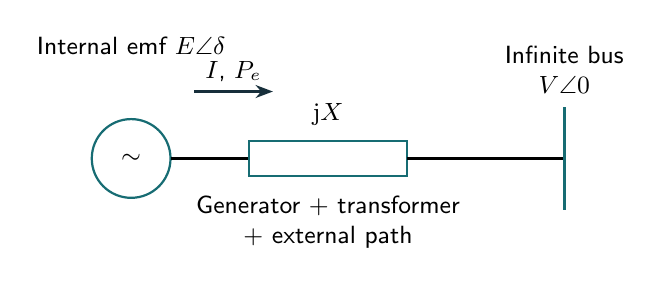
\begin{tikzpicture}[font=\small\sffamily]
\draw[thick,teal] (0,0) circle(.5);
\node at (0,0) {$\sim$};
\draw[thick] (.5,0)--(1.5,0);
\draw[thick,teal] (1.5,-.22) rectangle (3.5,.22);
\draw[thick] (3.5,0)--(5.5,0);
\draw[very thick,teal] (5.5,-.65)--(5.5,.65);
\node[above] at (0,1.2) {Internal emf $E\angle\delta$};
\node[above] at (2.5,.3) {$\jj X$};
\node[below,align=center] at (2.5,-.35) {Generator + transformer\\+ external path};
\node[above,align=center] at (5.5,.7) {Infinite bus\\$V\angle0$};
\draw[arr] (.8,.85)--(1.8,.85) node[midway,above] {$I$, $P_e$};
\end{tikzpicture}
\end{center}
\diagramcaption{For a classical first-swing transient study, use transient internal emf $E'$ behind $X'_d$ as appropriate. For a static synchronous model, the internal emf/reactance representation differs. Always state the chosen model; do not combine $E'$ with an unrelated reactance.}
\subsection{Derive the sine relation}
\[
I=\frac{Ee^{\jj\delta}-V}{\jj X}.
\]
The generator-side injected complex power in the per-unit three-phase convention is
\begin{align*}
S&=Ee^{\jj\delta}I^*
=\frac{\jj}{X}\left(E^2-EV e^{\jj\delta}\right)\\
&=\frac{EV}{X}\sin\delta
+\jj\frac{E^2-EV\cos\delta}{X}.
\end{align*}
Hence
\[
\ans{P_e=P_{\max}\sin\delta,\qquad P_{\max}=\frac{EV}{X}}.
\]
The active power at the other terminal has the same transferred magnitude because the path is lossless. The reactive injections at the two ends generally differ.
\begin{Caution}{Phase quantities, three-phase quantities and per unit}
For physical per-phase rms $E$ and $V$, total three-phase active power is $3EV\sin\delta/X$. In consistent three-phase per unit the compact relation is $EV\sin\delta/X$, without an extra factor of three. If physical line-to-line voltages are used instead, their product already contains the factor of three relative to phase voltages. State the convention before inserting values.
\end{Caution}
\par\noindent\begin{minipage}{\textwidth}
\input{Study_Assets/Module4/power_angle.tex}
\diagramcaption{A fixed transfer curve with $P_{\max}=2.2$ pu and $P_m=0.8$ pu. The low-angle intersection is restoring; the high-angle intersection is unstable in this classical model. The maximum is at $90^\circ$. This plot uses a single intact-network curve, not the different post-fault curve used later.}
\end{minipage}\par

\subsection{Equilibria and restoring action}
At a synchronous equilibrium, $P_m=P_e$. For $0<P_m<P_{\max}$ there are two intersections in $0<\delta<\pi$:
\[
\delta_s=\sin^{-1}\!\left(\frac{P_m}{P_{\max}}\right),\qquad
\delta_u=\pi-\delta_s.
\]
A small positive angle displacement from $\delta_s$ increases $P_e$. Then $P_m-P_e<0$, causing a restoring acceleration toward the original state. At $\delta_u$, the same displacement decreases $P_e$, so accelerating power becomes positive and the displacement grows.
\subsection{Synchronizing power coefficient}
For a small displacement $\Delta\delta$ about $\delta_0$,
\[
\Delta P_e\simeq K_s\Delta\delta,\qquad
\ans{K_s=\left.\frac{dP_e}{d\delta}\right|_{\delta_0}
=P_{\max}\cos\delta_0}.
\]
$K_s$ has units of pu power per electrical radian. With unchanged mechanical power, $\Delta P_a=-K_s\Delta\delta$. Positive $K_s$ supplies restoring action; negative $K_s$ supplies destabilizing action. Restoring action alone does not guarantee that an oscillation \emph{decays}: damping is a separate issue.
\subsection{What ``steady-state stability limit'' actually means}
For this lossless fixed-emf sine model,
\[
\ans{P_{\rm static,limit}=\frac{EV}{X},\quad\delta=90^\circ}.
\]
At the top of the curve $K_s=0$; there is no positive small-angle restoring margin. It is a limiting value, not a desirable normal operating point. For $P_m>P_{\max}$ there is no synchronous equilibrium on this curve.

Real operating limits can be lower because of heating, voltage restrictions, contingencies and required margin. A salient-pole model can introduce another angle term; resistance, excitation controls and a different network also change the simple curve. The syllabus's $EV/X$ result belongs to its stated classical assumptions.
\begin{Worked}{Example 1: transfer margin and synchronizing coefficient}
Let $E=1.1$, $V=1$, $X=0.5$ pu and $P_m=0.8$ pu. Then
\[
P_{\max}=2.2\ \mathrm{pu},\qquad
\delta_s=\sin^{-1}(0.8/2.2)=21.3237^\circ.
\]
The other equilibrium is $158.6763^\circ$. At the low-angle equilibrium,
\[
K_s=2.2\cos21.3237^\circ=2.04939\ \mathrm{pu/rad}.
\]
The difference between the curve maximum and operating power is $1.4$ pu. This is a model transfer margin, not a statement of permissible thermal loading or fault survivability. On a 100-MVA base, $0.8$ pu is 80 MW and the model maximum is 220 MW.
\end{Worked}
\checkq{Is the load-flow voltage angle at every bus the generator rotor angle $\delta$?}{No. A bus angle is the phase of its terminal voltage. The classical rotor angle is the phase of the generator's internal emf relative to the reference; the internal reactance generally creates a difference.}

\chapterstart{The swing equation, derived and interpreted}{swing}
\subsection{Start with mechanical torque}
For a rotor with moment of inertia $J$,
\[
J\frac{d^2\theta_m}{dt^2}=T_m-T_e.
\]
Here $\theta_m$ is absolute mechanical position. Write it as the synchronous motion plus a displacement:
\[
\theta_m=\omega_{ms}t+\delta_m,
\qquad \ddot\theta_m=\ddot\delta_m.
\]
Multiplying by the approximately synchronous mechanical speed gives
\[
J\omega_{ms}\ddot\delta_m\simeq P_m-P_e.
\]
This classical conversion uses $\omega_m\simeq\omega_{ms}$ during the swing; it does not assert that the rotor speed is exactly unchanged.
\subsection{Define inertia constant and convert the angle}
Stored kinetic energy at synchronous speed is $W_k=\tfrac12J\omega_{ms}^2$. Define
\[
\ans{H=\frac{W_k}{S_B}=\frac{\tfrac12J\omega_{ms}^2}{S_B}}.
\]
With $W_k$ in MJ and $S_B$ in MVA, $H$ is in seconds. It expresses stored kinetic energy per unit rated apparent power. Do not confuse the inertia constant $H$ with the moment of inertia $J$.

For a $p$-pole machine,
\[
\delta=\frac p2\delta_m,\qquad
\omega_s=\frac p2\omega_{ms}=2\pi f_s.
\]
Divide the torque-derived power equation by $S_B$ and substitute $H$. The electrical-angle swing equation is
\[
\ans{\frac{2H}{\omega_s}\frac{d^2\delta}{dt^2}=P_m-P_e=P_a}.
\]
Powers are pu on the base used for $H$, and $\delta$ is in electrical radians. The coefficient $M=2H/\omega_s$ is often introduced to shorten the expression to $M\ddot\delta=P_a$.
\subsection{Radian and degree forms}
With $\omega_s=2\pi f_s$,
\[
\frac{H}{\pi f_s}\ddot\delta_{rad}=P_a.
\]
Because $\delta_{rad}=(\pi/180)\delta_{deg}$,
\[
\ans{\frac{H}{180f_s}\ddot\delta_{deg}=P_a}.
\]
Use the degree form only when the differentiated angle is in electrical degrees. The $\sin\delta$ power law and energy integrals must also be evaluated with a consistent angle convention.
\subsection{Speed, acceleration and angle are different}
\[
\dot\delta=\Delta\omega_e,\qquad
\omega_e=\omega_s+\dot\delta,\qquad
\Delta f=\frac{\dot\delta}{2\pi}.
\]
$P_a>0$ means relative speed is increasing. $P_a<0$ means relative speed is decreasing. It does \emph{not} necessarily mean that the rotor angle is already decreasing: if $\dot\delta>0$, the angle still rises during deceleration until the excess speed reaches zero.

At $P_a=0$, acceleration is zero. The rotor can still have nonzero excess speed and continue moving relative to the synchronous reference. At a maximum-angle turning point, $\dot\delta=0$; to turn back, the accelerating power is normally negative there.
\begin{center}
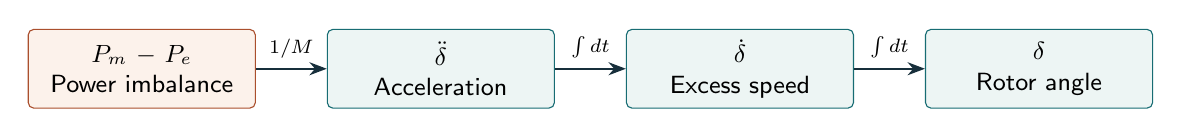
\begin{tikzpicture}[node distance=9mm]
\node[hot] (p) {$P_m-P_e$\\Power imbalance};
\node[block,right=of p] (a) {$\ddot\delta$\\Acceleration};
\node[block,right=of a] (w) {$\dot\delta$\\Excess speed};
\node[block,right=of w] (d) {$\delta$\\Rotor angle};
\draw[arr] (p)--(a) node[midway,above,font=\scriptsize] {$1/M$};
\draw[arr] (a)--(w) node[midway,above,font=\scriptsize] {$\int dt$};
\draw[arr] (w)--(d) node[midway,above,font=\scriptsize] {$\int dt$};
\end{tikzpicture}
\end{center}
\diagramcaption{An abrupt fault can abruptly change electrical power and acceleration. Without an impulse torque, neither rotor angle nor rotor speed jumps at fault application or clearing.}
\subsection{Common-base conversion}
Stored physical energy is unchanged by choosing another per-unit base. Therefore
\[
\ans{H_{new}=H_{old}\frac{S_{old}}{S_{new}}}.
\]
For the same physical machine, larger power base means smaller numerical $H$. Convert $P_m$, $P_e$ and $H$ together. For coherently moving machines referred to a common frequency, their stored energies add; the equivalent inertia on $S_B$ is $H_{eq}=\sum_i H_i S_i/S_B$. Arbitrary machines with different angles cannot simply be collapsed into one swing without a justified equivalent model.
\begin{Worked}{Example 2: acceleration, speed and angle}
A 100-MVA machine has $H=5$ s at 50 Hz. For 0.1 s suppose the approximately constant power imbalance is $P_a=0.2$ pu and initial excess speed is zero.
\[
\ddot\delta=\frac{2\pi50}{2(5)}(0.2)
=6.283185\ \mathrm{rad/s^2}.
\]
After 0.1 s,
\[
\dot\delta=0.628319\ \mathrm{rad/s},\quad
\Delta f=0.100000\ \mathrm{Hz},
\]
\[
\Delta\delta=\tfrac12(6.283185)(0.1)^2
=0.0314159\ \mathrm{rad}=1.8^\circ.
\]
Stored synchronous kinetic energy is $5\times100=500$ MJ. On a 200-MVA base, $H=2.5$ s and the same 20-MW imbalance is $0.1$ pu. Their ratio gives exactly the same physical acceleration. A constant $P_a$ is an assumption of this illustration, not the usual sine-dependent post-fault power.
\end{Worked}
\subsection{The classical assumptions and their limits}
For a first-swing SMIB calculation, commonly assume constant mechanical input over the short interval, constant transient internal emf, fixed infinite-bus voltage/frequency, a lossless reduced network and negligible damping. A fault changes the applicable electrical-power curve. The pre-fault, fault-on and post-fault curves can have different maxima.

A damped extension is $M\ddot\delta+D\dot\delta=P_m-P_e$, with $D$ defined in the compatible power-per-speed units. Detailed models can include excitation, governor and turbine dynamics, saliency and multiple machines. State the model rather than silently applying the classical equation to every situation.
\checkq{Immediately after fault clearance $P_e>P_m$. Why can the rotor angle still increase?}{The rotor has accumulated positive excess speed. Negative accelerating power reduces that speed; the angle continues to rise until the excess speed becomes zero.}

\chapterstart{Dynamic stability: synchronizing action and damping}{dynamic}
\subsection{Linearize about a synchronous equilibrium}
Set $\delta=\delta_0+\Delta\delta$ and suppose $P_{m0}=P_e(\delta_0)$. For a small disturbance and locally constant controls,
\[
\ans{M\Delta\ddot\delta+D\Delta\dot\delta+K_s\Delta\delta
=\Delta P_m},\qquad M=\frac{2H}{\omega_s}.
\]
The restoring coefficient is $K_s=P_{\max}\cos\delta_0$ for the classical sine curve. The homogeneous equation explains the local response:
\begin{itemize}
\item $K_s>0$, $D>0$: restoring action and positive damping; perturbations decay in this simple model.
\item $K_s>0$, $D=0$: restoring action but no decay; small oscillations persist.
\item $K_s>0$, $D<0$: the oscillation can grow even though the static power-angle slope is positive.
\item $K_s<0$: no restoring equilibrium; damping alone does not repair a negative static stiffness in this model.
\end{itemize}
\subsection{Optional mathematical view}
The characteristic equation is $M\lambda^2+D\lambda+K_s=0$. For $K_s>0$,
\[
\omega_n=\sqrt{K_s/M},\qquad
\zeta=\frac{D}{2\sqrt{MK_s}}.
\]
With no damping the roots are $\pm\jj\omega_n$. Positive damping moves the stable roots into the left half-plane. These expressions are a helpful interpretation of the syllabus's dynamic-stability topic; they are not a replacement for a full control-system model.
\par\noindent\begin{minipage}{\textwidth}
\input{Study_Assets/Module4/damping.tex}
\diagramcaption{Conceptual linear responses with positive, zero and negative damping. Traces are vertically offset for readability and do not represent absolute rotor angles or a particular machine simulation. All illustrate a positive synchronizing coefficient; growing oscillations are possible despite a positive static slope.}
\end{minipage}\par

\subsection{Why excitation and a power-system stabilizer matter}
An excitation system regulates generator voltage and affects electrical torque. Its dynamics can change both synchronizing and damping torque. Fast high-gain excitation can help voltage support yet reduce damping in some operating conditions; increased gain is not an automatic cure for all stability problems.

A \textbf{power-system stabilizer (PSS)} adds a suitably phased supplementary signal to excitation, commonly based on speed/frequency or power changes, to contribute damping to electromechanical oscillations. Its purpose is to oppose oscillatory motion through electrical torque. The relevant damping depends on the entire machine, controller and network combination.
\begin{Idea}{Remember the distinction}
$K_s$ answers: does an angle displacement create a restoring torque? Damping answers: does the oscillation lose energy and settle? A system can have restoring action while its oscillations grow because its effective damping is negative.
\end{Idea}

\chapterstart{Transient stability and the equal-area criterion}{eac}
\subsection{Three networks during a fault}
Before the fault, $P_m=P_{pre}(\delta_0)$ and $\dot\delta_0=0$. During the fault, electrical transfer often falls sharply, so $P_m-P_{fault}>0$ and the rotor accelerates. After breakers clear the fault, transfer recovers according to the \emph{post-fault} network. Clearing may permanently remove a circuit, so the final curve need not equal the original curve.
\begin{center}
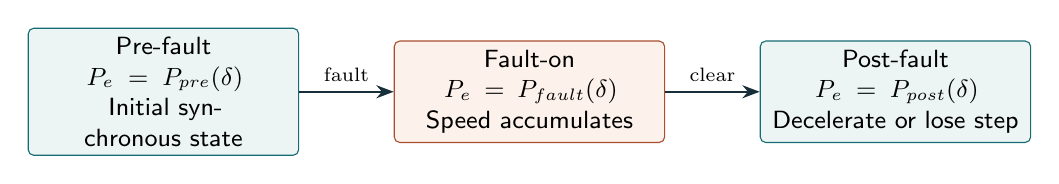
\begin{tikzpicture}[node distance=12mm]
\node[block,text width=3.2cm] (pre) {Pre-fault\\$P_e=P_{pre}(\delta)$\\Initial synchronous state};
\node[hot,text width=3.2cm,right=of pre] (fault) {Fault-on\\$P_e=P_{fault}(\delta)$\\Speed accumulates};
\node[block,text width=3.2cm,right=of fault] (post) {Post-fault\\$P_e=P_{post}(\delta)$\\Decelerate or lose step};
\draw[arr] (pre)--(fault) node[midway,above,font=\scriptsize] {fault};
\draw[arr] (fault)--(post) node[midway,above,font=\scriptsize] {clear};
\end{tikzpicture}
\end{center}
\diagramcaption{At each switch, angle and speed are continuous. Power and acceleration can change abruptly. Fault clearing is the interruption of fault current by the protection/breaker system, not merely the instant when the relay first detects the fault.}
\subsection{Derive the area relation from the swing equation}
With no damping and a fixed power curve within a time interval,
\[
M\ddot\delta=P_m-P_e(\delta).
\]
Multiply by $\dot\delta$ and integrate:
\begin{align*}
M\ddot\delta\,\dot\delta&=(P_m-P_e)\dot\delta,\\
\ans{\frac M2\left(\dot\delta^2-\dot\delta_0^2\right)}
&=\ans{\int_{\delta_0}^{\delta}(P_m-P_e(\alpha))\,d\alpha}.
\end{align*}
This first integral is an energy-like balance for motion relative to the synchronous reference. Positive area increases squared excess speed; negative area reduces it. The areas use electrical \textbf{radians} and have units pu power times radian. They are not a literal number of joules without conversion; the relation above shows the scaling.

Starting with zero excess speed, a first-swing turning point also has zero excess speed. The net signed area from the initial state to that point must therefore be zero. This is the origin of the \textbf{equal-area criterion (EAC)}.
\subsection{Actual and available decelerating area are different}
In the common fault case, let $\delta_c$ be clearing angle and suppose the post-fault curve is above $P_m$ immediately after clearing. Define
\[
A_{acc}=\int_{\delta_0}^{\delta_c}(P_m-P_{fault})\,d\delta,
\]
\[
A_{dec,actual}=\int_{\delta_c}^{\delta_{max}}(P_{post}-P_m)\,d\delta.
\]
At a successful undamped first-swing turning point,
\[
\ans{A_{acc}=A_{dec,actual}}.
\]
Let $\delta_u$ be the unstable post-fault intersection. The maximum available decelerating area before reaching that boundary is
\[
A_{dec,available}=\int_{\delta_c}^{\delta_u}(P_{post}-P_m)\,d\delta.
\]
A strictly stable first swing has $A_{acc}<A_{dec,available}$ and turns at $\delta_{max}<\delta_u$. At the critical boundary the two \emph{available-limit} areas are equal; the ideal undamped trajectory approaches the unstable equilibrium with zero speed. Greater accelerating area carries the rotor through the boundary and it loses synchronism.
\begin{Caution}{Avoid two misleading shortcuts}
Do not say that a stable swing has $A_{acc}<A_{dec,actual}$: its actual areas are equal at the turning point. The strict comparison is against the \emph{available} area. Also, if clearing occurs while $P_{post}<P_m$, the rotor continues accelerating after clearing until the post-fault curve crosses $P_m$. Include that extra positive area; do not label the whole post-fault interval as deceleration.
\end{Caution}
\par\noindent\begin{minipage}{\textwidth}
\input{Study_Assets/Module4/equal_area.tex}
\diagramcaption{An independently calculated stable example: $P_m=0.8$ pu, pre-fault maximum 2.2 pu, fault-on transfer zero, post-fault maximum 1.375 pu. Clearing at $55^\circ$ gives a turning angle $107.6245^\circ$. The rust accelerating area equals the teal actual decelerating area. The post-fault unstable intersection is $144.4215^\circ$, beyond the turning point.}
\end{minipage}\par

\subsection{What the criterion establishes}
In the classical undamped SMIB model, equal-area analysis decides first-swing synchronism without solving every time step. A stable undamped machine subsequently oscillates rather than settling; physical positive damping is needed for decay. Repeated switching and later swings can require additional analysis.

A two-machine system can sometimes be reduced to an equivalent relative-angle problem. A general multi-machine system has several coupled angles and does not automatically admit one universal shaded-area test. Damping, time-dependent controls and changing mechanical input also alter the simple conservative criterion.
\subsection{Why \texorpdfstring{$90^\circ$}{90 degrees} is not the transient trip boundary}
The static sine curve peaks at $90^\circ$, but the rotor can swing past that angle and still turn back before the unstable post-fault equilibrium. In the plotted example, $\delta_{max}=107.6245^\circ$ is a stable first swing. Stability depends on the accumulated speed/energy and the remaining decelerating area, not solely on crossing the top of the curve.
\checkq{A post-fault equilibrium exists because $P_m<P_{post,max}$. Is that enough for transient stability?}{No. The rotor may reach the post-fault network with too much excess speed. It must have enough available decelerating area to stop before the unstable boundary.}

\chapterstart{Critical clearing angle and clearing time}{critical}
\subsection{The fault is cleared, but one path is lost}
Let the pre-fault, fault-on and post-fault electrical powers be
\[
P_{pre}=P_1\sin\delta,\qquad
P_{fault}=P_f\sin\delta,\qquad
P_{post}=P_2\sin\delta.
\]
Assume constant $P_m$, initial synchronous operation and the classical undamped model. Then
\[
\delta_0=\sin^{-1}(P_m/P_1),\qquad
\delta_u=\pi-\sin^{-1}(P_m/P_2).
\]
The low-angle initial equilibrium is assumed. A post-fault equilibrium requires $P_m<P_2$; otherwise the usual decelerating boundary used here does not exist.
\subsection{Derive the critical angle for a zero-transfer fault}
For $P_f=0$, accelerating area up to the critical clearing angle is
\[
A_{acc}=P_m(\delta_{cr}-\delta_0).
\]
At the boundary, use all the available decelerating area:
\begin{align*}
A_{dec,available}
&=\int_{\delta_{cr}}^{\delta_u}(P_2\sin\delta-P_m)\,d\delta\\
&=P_2(\cos\delta_{cr}-\cos\delta_u)
-P_m(\delta_u-\delta_{cr}).
\end{align*}
Equate the areas and collect terms:
\[
P_2(\cos\delta_{cr}-\cos\delta_u)=P_m(\delta_u-\delta_0),
\]
\[
\ans{\cos\delta_{cr}=\cos\delta_u+\frac{P_m}{P_2}(\delta_u-\delta_0)}.
\]
Angles in the linear difference must be \textbf{radians}. Take the physically relevant root in the fault trajectory. If the expression lies outside $[-1,1]$ or gives an angle inconsistent with the assumed sequence, do not force an inverse-cosine answer: check feasibility and assumptions. A system can be unstable even for immediate switching to a weakened network.
\subsection{Convert the critical angle into time: a special constant-acceleration case}
During a zero-transfer fault,
\[
\ddot\delta=\frac{\omega_sP_m}{2H}.
\]
With initial excess speed zero and fault application at $t=0$,
\[
\delta_c-\delta_0=\frac{\omega_sP_m}{4H}t_c^2.
\]
Thus
\[
\ans{t_{cr}=\sqrt{\frac{4H(\delta_{cr}-\delta_0)}{\omega_sP_m}}}.
\]
Use electrical radians and seconds. This formula assumes $P_e=0$ throughout the fault and constant $P_m$. It is not a general clearing-time formula when fault-on transfer is nonzero or controls make the power time dependent.
\subsection{General sinusoidal fault-on transfer}
If $P_f$ is nonzero, equating areas gives
\[
P_m(\delta_{cr}-\delta_0)+P_f(\cos\delta_{cr}-\cos\delta_0)
=P_2(\cos\delta_{cr}-\cos\delta_u)-P_m(\delta_u-\delta_{cr}),
\]
\[
\ans{\cos\delta_{cr}=\frac{P_m(\delta_u-\delta_0)+P_2\cos\delta_u-P_f\cos\delta_0}{P_2-P_f}}.
\]
This expression needs $P_2\ne P_f$ and the assumed physically applicable trajectories. If fault-on and post-fault curves are the same, changing the nominal clearing instant does not improve transfer in this model; inspect the energy balance directly instead of dividing by zero.

For nonzero $P_f$, acceleration depends on angle. Obtain time by integrating the swing equation, or use the first integral to write, during a monotonically increasing fault-on swing,
\[
t_c=\int_{\delta_0}^{\delta_c}
\frac{d\delta}{\sqrt{\dfrac{\omega_s}{H}
\int_{\delta_0}^{\delta}(P_m-P_f\sin\alpha)\,d\alpha}}.
\]
The apparent endpoint singularity is integrable when initial accelerating power is positive. Numerical time integration is generally more convenient. Do not insert the nonzero-fault critical angle into the zero-transfer time formula.
\begin{Idea}{What changes with inertia?}
In this fixed-power-curve classical model, the critical angle follows from the areas and is independent of $H$. Larger $H$ makes the trajectory take longer to reach that angle. For the zero-transfer case $t_{cr}\propto\sqrt H$. This increases time allowance; it does not raise the sine curve's $EV/X$ maximum.
\end{Idea}

\chapterstart{Worked transient-stability applications}{applications}
\subsection{Example 3: fault clearing with a permanently weakened network}
All examples in this stability half are independently constructed teaching examples. Use $E=1.1$, $V=1$, $X_{pre}=0.5$, $X_{post}=0.8$ pu, $P_m=0.8$ pu, $H=5$ s and $f_s=50$ Hz. Suppose a severe fault makes electrical transfer zero until clearing; after clearing a path remains disconnected.
\subsubsection{Step 1: calculate the three curves and intersections}
\[
P_1=1.1/0.5=2.2,\qquad P_f=0,\qquad P_2=1.1/0.8=1.375\ \mathrm{pu}.
\]
\[
\delta_0=\sin^{-1}(0.8/2.2)=21.323686^\circ=0.372168534\ \mathrm{rad}.
\]
The post-fault stable equilibrium is $\delta_s=35.578526^\circ$; the unstable boundary is
\[
\delta_u=180^\circ-35.578526^\circ=144.421474^\circ.
\]
The post-fault equilibrium exists, but that fact alone does not establish survival of the fault.
\subsubsection{Step 2: calculate the critical angle}
\[
\cos\delta_{cr}=\cos\delta_u+
\frac{0.8}{1.375}(\delta_u-\delta_0).
\]
Evaluate the difference in radians to obtain
\[
\ans{\delta_{cr}=1.118874537\ \mathrm{rad}=64.106789^\circ}.
\]
The accelerating area at this boundary is
\[
0.8(1.118874537-0.372168534)=0.5973648\ \mathrm{pu\cdot rad}.
\]
Direct evaluation of the available post-fault integral gives the same value. This independently checks the inverse-cosine calculation.
\subsubsection{Step 3: calculate the critical time}
\[
\omega_s=2\pi(50)=314.159265\ \mathrm{rad/s},
\]
\[
\ans{t_{cr}=\sqrt{\frac{4(5)(1.118874537-0.372168534)}{314.159265(0.8)}}
=0.243764\ \mathrm{s}}.
\]
This is an ideal model boundary, not a recommended relay setting. The actual fault-clearing interval includes detection/relay action and breaker interruption; practical coordination needs margin below the computed boundary and attention to the actual operating condition.
\subsubsection{Step 4: check a clearing angle of $55^\circ$}
For $\delta_c=55^\circ=0.959931089$ rad,
\[
A_{acc}=0.8(0.959931089-0.372168534)=0.4702100.
\]
The corresponding zero-transfer fault duration is $t_c=0.216270$ s, below $t_{cr}$. Solve for the actual turning point from
\[
0.4702100=1.375(\cos55^\circ-\cos\delta_{max})
-0.8(\delta_{max}-0.959931089).
\]
The first relevant root is
\[
\ans{\delta_{max}=107.624509^\circ<144.421474^\circ}.
\]
This is the stable shaded-area case in Section~\ref{eac}. It also demonstrates why crossing $90^\circ$ is not, by itself, proof of a transient loss of synchronism.
\subsubsection{Step 5: compare two actual time trajectories}
\par\noindent\begin{minipage}{\textwidth}
\input{Study_Assets/Module4/swing_response.tex}
\diagramcaption{Numerical integration of the same undamped classical swing equation, using a fourth-order Runge--Kutta step of 0.0005 s. Clearing after 0.19 s gives a bounded first swing (maximum about $92.66^\circ$); clearing after 0.27 s crosses the post-fault unstable boundary and the angle continues advancing. The model boundary is 0.243764 s. The unstable trace is truncated vertically to keep the comparison readable.}
\end{minipage}\par

\subsection{Example 4: some electrical transfer survives during the fault}
Keep Example 3's pre-fault and post-fault data, but set $P_f=0.4$ pu. The critical-angle relation gives
\[
\cos\delta_{cr}=
\frac{0.8(\delta_u-\delta_0)+1.375\cos\delta_u-0.4\cos\delta_0}{1.375-0.4},
\]
\[
\ans{\delta_{cr}=76.486083^\circ}.
\]
The initial fault-on accelerating power is $0.8-0.4\sin\delta_0=0.654545$ pu rather than 0.8 pu. Transfer surviving during the fault reduces accumulated acceleration and changes the allowable angle. Time must be calculated from the nonconstant-acceleration trajectory. This example deliberately stops at the angle rather than applying an invalid constant-acceleration time formula.
\subsection{Example 5: a sudden increase in mechanical input}
A fault is not necessary for a transient swing. Suppose $P_e=2\sin\delta$ remains unchanged, but $P_m$ steps from 0.6 to 1.0 pu. Initially
\[
\delta_0=\sin^{-1}(0.6/2)=17.457603^\circ.
\]
After the step, the new stable intersection is $\delta_s=30^\circ$ and the unstable intersection is $\delta_u=150^\circ$. From $\delta_0$ to $30^\circ$, the new mechanical input exceeds electrical output, so the rotor accelerates. The area is
\begin{align*}
A_{acc}&=\int_{\delta_0}^{\pi/6}(1-2\sin\delta)\,d\delta\\
&=(\pi/6-\delta_0)+2(\cos(\pi/6)-\cos\delta_0)\\
&=0.04307853\ \mathrm{pu\cdot rad}.
\end{align*}
Maximum available deceleration on the unchanged curve is
\[
A_{dec,available}=\int_{\pi/6}^{5\pi/6}(2\sin\delta-1)\,d\delta
=1.36970651.
\]
It exceeds the accelerating area, so this first swing is stable. The rotor does not stop at $30^\circ$: it has positive excess speed there. The actual turning point satisfies
\[
2\big(\cos30^\circ-\cos\delta_{max}\big)
-(\delta_{max}-\pi/6)=0.04307853,
\]
\[
\ans{\delta_{max}=43.098500^\circ}.
\]
With positive damping, subsequent oscillations settle about $30^\circ$. With the ideal no-damping assumption, they persist.
\subsection{Application to a sudden line outage}
A line opening increases the effective transfer reactance, reducing the power-angle maximum even if there is no preceding fault interval. Immediately after opening, the initial angle and speed are unchanged, but electrical power is lower. The rotor may accelerate until it reaches the new stable intersection, then needs sufficient area to decelerate before the new unstable boundary.

This has the same signed-area logic as the input-step example, with the \emph{electrical curve} changing instead of the mechanical input line. Merely verifying $P_m<P_{post,max}$ is insufficient. An abrupt switch can introduce a transient energy excursion even when both pre-outage and post-outage equilibria exist.
\subsection{A reliable equal-area problem-solving sequence}
\begin{enumerate}
\item Identify the base, internal emf model, mechanical input and fault/network sequence.
\item Reduce the relevant network reactances to obtain pre-fault, fault-on and post-fault transfer curves. Do not presume every fault gives $P_e=0$.
\item Find the initial stable equilibrium and the post-fault stable/unstable intersections.
\item Mark intervals where $P_m-P_e$ is positive or negative. Include any acceleration after clearing.
\item Write the signed integrals in radians. For a critical angle, stop available deceleration at the post-fault unstable boundary.
\item Solve for the physically applicable angle; check the root and compare actual/available areas.
\item Convert angle to time only using the appropriate fault-on swing equation. State all assumptions and interpret the result with a practical margin.
\end{enumerate}

\chapterstart{Improving stability limits}{improvements}
Different measures improve different parts of the problem. Raising $P_{\max}$ improves electrical transfer strength; reducing fault-on time limits accelerating energy; adding damping reduces oscillations. Do not treat these as interchangeable.
\begin{center}\small\begin{longtable}{L{.23\textwidth}L{.40\textwidth}L{.28\textwidth}}
\toprule Measure & Physical reason & Qualification\\\midrule\endhead
Faster protection and breaker interruption & Shorter fault duration lowers the accumulated accelerating area and excess speed. & Count the actual clearing time, including the breaker. Backup operation can be slower.\\
Stronger transmission paths / parallel circuits & Lower effective $X$ raises $EV/X$ and available transfer/deceleration. & Use the surviving topology after the contingency; a tripped parallel circuit is no longer available.\\
Series compensation & Reduces effective series reactance and can improve transfer. & Detailed application must consider protection and oscillatory interactions, including subsynchronous resonance.\\
Voltage support and suitable excitation & Sustains $V$ and internal emf, supporting synchronizing power and post-fault electrical torque. & Controller dynamics matter; higher excitation gain alone need not improve damping.\\
Power-system stabilizer & Adds properly phased damping torque through excitation. & Requires suitable tuning for relevant modes and operating conditions.\\
Fast mechanical-power reduction & Fast valving or other appropriate control reduces $P_m$, hence fault/post-fault accelerating power. & The mechanism and achievable speed depend on the prime mover and controls.\\
Dynamic braking & A temporary electrical braking load extracts additional power/energy during the swing. & Requires equipment designed for the energy and switching duty.\\
High-speed reclosing where appropriate & Restoration of a healthy path can restore a stronger transfer curve. & Appropriate only under suitable fault, equipment and reclosing conditions; a permanent fault may recur.\\
Larger effective inertia & Reduces acceleration for a given physical imbalance and can provide more clearing-time allowance. & Does not by itself raise the fixed sine transfer maximum or critical angle.\\
Reduced initial transfer / operating margin & Lower initial loading can reduce the initial angle and improve contingency survival margin. & Recompute the complete curves and disturbance; margin is system dependent.\\\bottomrule
\end{longtable}\end{center}
\subsection{Relate this to Module 3 protection}
A relay decides that its fault criterion is satisfied and sends a trip command. The breaker then opens and interrupts current. Stability benefits from removal of the fault before the critical boundary, whereas selectivity requires the appropriate equipment to trip. Protection coordination balances prompt primary clearing with correctly coordinated backup; delayed clearing can materially change transient survival.
\subsection{Relate this to Module 2 line parameters}
An increased transmission reactance reduces $P_{\max}$ in the simple SMIB equivalent. Parallel paths can reduce the effective reactance. Compensation and voltage regulation affect transfer capability, but must be modelled consistently with the network and machine representation. The practical limit also respects thermal/voltage constraints and the actual contingency.
\checkq{Which improves the ideal critical angle: doubling $H$ or strengthening the post-fault network?}{With the same classical power curves, doubling $H$ changes time allowance but not the area-derived angle. Strengthening the post-fault network changes its curve and available deceleration, so it can improve the angle margin.}

\chapterstart{Revision sheet and exam preparation}{revision}
\subsection{Essential equations with their assumptions}
\begin{center}\small\begin{longtable}{L{.43\textwidth}L{.48\textwidth}}
\toprule Equation & Meaning / condition\\\midrule\endhead
$S_i=P_i+\jj Q_i=V_iI_i^*$ & Net injection; load demand enters with negative sign after subtracting from generation.\\
$\boldsymbol I=Y_{bus}\boldsymbol V$ & Balanced network model on consistent bases; includes relevant taps and shunts.\\
$Y_{ii}=\sum y_{ik}+y_{i,sh}$; $Y_{ij}=-y_{ij}$ & Simple reciprocal series branches plus bus/terminal shunts. Use modified stamps for off-nominal transformers.\\
$P_i=\sum_j|V_i||V_j|(G_{ij}\cos\theta_{ij}+B_{ij}\sin\theta_{ij})$ & Nonlinear active-injection equation.\\
$Q_i=\sum_j|V_i||V_j|(G_{ij}\sin\theta_{ij}-B_{ij}\cos\theta_{ij})$ & Nonlinear reactive-injection equation.\\
$V_i^{k+1}=\dfrac{1}{Y_{ii}}\!\left[\dfrac{P_i-\jj Q_i}{(V_i^k)^*}-\sum_{j<i}Y_{ij}V_j^{k+1}-\sum_{j>i}Y_{ij}V_j^k\right]$ & GS PQ update in the chosen order; fixed slack always retained.\\
$P_e=(EV/X)\sin\delta$ & Classical lossless, non-salient SMIB; per-unit convention.\\
$P_{\max}=EV/X$, $K_s=P_{\max}\cos\delta_0$ & Fixed curve's static maximum and local synchronizing coefficient.\\
$H=\tfrac12J\omega_{ms}^2/S_B$ & Synchronous stored energy per rating/base; seconds.\\
$\dfrac{2H}{\omega_s}\ddot\delta=P_m-P_e$ & Electrical radians; powers on the same base as $H$.\\
$\dfrac{H}{180f_s}\ddot\delta_{deg}=P_m-P_e$ & Alternative electrical-degree form.\\
$H_{new}=H_{old}S_{old}/S_{new}$ & Same stored physical energy, different power base.\\
$M\Delta\ddot\delta+D\Delta\dot\delta+K_s\Delta\delta=0$ & Small-disturbance homogeneous motion in the local constant-coefficient model.\\
$\frac M2(\dot\delta^2-\dot\delta_0^2)=\int(P_m-P_e)d\delta$ & Undamped swing first integral; angle in radians; fixed applicable power curve per interval.\\
$\delta_u=\pi-\sin^{-1}(P_m/P_2)$ & Unstable intersection of the sinusoidal post-fault curve, for $0<P_m<P_2$.\\
$\cos\delta_{cr}=\cos\delta_u+(P_m/P_2)(\delta_u-\delta_0)$ & Zero-transfer fault; initial synchronous state and specified post-fault curve.\\
$t_{cr}=\sqrt{4H(\delta_{cr}-\delta_0)/(\omega_sP_m)}$ & Zero electrical transfer during fault; constant mechanical input; radians.\\\bottomrule
\end{longtable}\end{center}
\subsection{Bus classification in one glance}
\begin{center}\begin{tabularx}{\textwidth}{L{.22\textwidth}Y Y}
\toprule Bus & Specified & Calculated\\\midrule
PQ & $P,Q$ & $|V|,\theta$\\
PV & $P,|V|$ & $Q,\theta$\\
Slack & $|V|,\theta$ & $P,Q$\\\bottomrule
\end{tabularx}\end{center}
Use one angle reference per connected island in the ordinary single-slack formulation. A slack bus balances losses/injection mismatch; it is not physical earth. A PV bus that reaches a reactive capability limit can be treated as PQ with Q fixed at the applicable limit and voltage magnitude free.
\subsection{Short-answer prompts with model points}
\begin{enumerate}
\item \textbf{Why load flow?} Determine steady-state bus voltages, generator requirements and branch flows for a specified network and loading; check voltage, capability and flow limits.
\item \textbf{Why a slack bus?} Choose angle reference and calculate balancing active/reactive injection because losses are unknown before voltages/flows are solved.
\item \textbf{Explain Y-bus signs.} The branch current $y(V_i-V_j)$ contributes $+y$ to the diagonal and $-y$ to the off-diagonal. Shunts add to diagonals.
\item \textbf{What makes GS sequential?} The latest updated voltages are used immediately in later bus substitutions within the same sweep.
\item \textbf{Why estimate Q at a PV bus?} Q is an output needed to sustain the specified magnitude; it must be calculated and checked against generator capability.
\item \textbf{Define an infinite bus.} An ideal reference with voltage magnitude and frequency unaffected by the studied machine's power exchange.
\item \textbf{Define $H$.} Synchronous stored rotor kinetic energy divided by rated/base apparent power; seconds, or equivalently MJ/MVA.
\item \textbf{State the steady-state limit.} For the lossless fixed-emf non-salient SMIB model, $EV/X$ at $90^\circ$, where synchronizing slope becomes zero.
\item \textbf{State EAC correctly.} For an undamped classical SMIB first swing from rest, accelerating area equals actual decelerating area at the turning point; stability requires enough available deceleration before the unstable boundary.
\item \textbf{What is critical clearing time?} The maximum fault duration at the stability boundary for the stated system, disturbance and model. Practical clearing needs margin.
\item \textbf{Why distinguish dynamic and transient?} Small-disturbance damping/control response and large-disturbance nonlinear synchronism address different behaviour; do not identify every growing oscillation with a severe fault.
\item \textbf{Name improvements and mechanisms.} Faster clearing limits acceleration; smaller X/voltage support strengthens transfer; PSS improves damping; fast input reduction or braking lowers net accelerating energy.
\end{enumerate}
\subsection{Long-answer structures}
\textbf{Network/Y-bus question:} draw the per-phase network; define injections and admittances; apply KCL at each bus; assemble self/mutual terms; include shunts/taps; state conditional properties; verify the class three-bus matrix.

\textbf{Qualitative Gauss--Seidel question:} identify PQ/PV/slack data; derive the substitution from $S=VI^*$ and $I=YV$; describe flat start and newest-value use; explain PQ/PV updates and Q limits; give the flowchart; explain tolerance/mismatch checks and suitable acceleration; list merits/limitations. Extensive iteration tables are outside the stipulated numerical requirement.

\textbf{Power-angle/swing question:} draw SMIB with consistent internal emf/reactance; derive $P_e$; identify stable/unstable intersections and $K_s$; start from rotor torque, introduce synchronous displacement and $H$; convert mechanical to electrical angle; give units and interpret acceleration, speed and angle.

\textbf{Equal-area/application question:} state classical assumptions; multiply the swing equation by speed and integrate; draw pre/fault/post curves; distinguish actual from available deceleration; identify $\delta_u$; equate critical areas; derive time only for zero fault-on transfer; explain practical fault-clearing margin and methods of improvement.

\chapterstart{Practice questions and explained answers}{practice}
Cover the answers and explain your reasoning before checking. Numerical Gauss--Seidel work remains optional; its required qualitative understanding is tested here instead.
\subsection{Concept checks}
\begin{enumerate}
\item \textbf{A generator bus has fixed P and Q. Is it automatically PV?} No. Type follows specified constraints, not the presence of generation. Fixed net P and Q define PQ.
\item \textbf{A load exists at a PV bus. Which P enters GS?} Net active injection $P_G-P_L$. The computed net Q is $Q_G-Q_L$; add local load Q when checking generator capability.
\item \textbf{Are both slack power and voltage unknown?} No. Slack magnitude/angle are specified; active/reactive injections are outputs in the ordinary formulation.
\item \textbf{Can disconnected islands share one angle reference through Y-bus?} No. Each island needs a reference and feasible power balance/control arrangement. No physical branch couples their absolute angles.
\item \textbf{Must every Y-bus be symmetric?} No. Ordinary reciprocal branches give symmetry, but complex phase-shifting tap stamps can give unequal off-diagonals. Transpose symmetry is distinct from conjugate-transpose symmetry.
\item \textbf{Must a diagonal have the greatest magnitude?} No. Complex cancellation and shunts make that blanket claim invalid. Construct entries from the actual branches.
\item \textbf{What does the class example's zero row sum mean?} With no shunts/off-nominal taps, a common bus voltage drives no series current. Realistic Y-bus matrices need not have zero row sums.
\item \textbf{Which own-bus voltage is in a GS denominator?} Its current pre-update estimate, conjugated. Earlier buses in the sum use their newest values.
\item \textbf{What does PV magnitude restoration preserve?} The newly estimated phase. Multiplying by $|V_i|^{spec}/|\widetilde V_i|$ changes magnitude without changing phase.
\item \textbf{Can PV voltage control demand unlimited Q?} No. At a generator reactive limit, fix Q at that limit and allow magnitude to vary under the adopted PQ treatment.
\item \textbf{Do tiny voltage changes always prove a valid solution?} Check specified-power residuals too. A stagnant iteration can retain material mismatch.
\item \textbf{Is 1.6 universally the best acceleration factor?} No. Performance and convergence depend on the nonlinear problem and update scheme.
\item \textbf{At a stable equilibrium is $P_m-P_e>0$?} No, it is zero. Examine restoring response to a displacement.
\item \textbf{If $P_m>P_{\max}$, can inertia create an equilibrium?} No. Inertia slows motion but cannot supply a missing electrical-power intersection.
\item \textbf{Does positive $K_s$ imply settling?} No. Positive damping is also needed in the simple linear model; zero damping permits persistent oscillations and negative damping can cause growth.
\item \textbf{If $P_a=0$ at an instant, is excess speed zero?} Not necessarily. Zero acceleration does not imply zero velocity.
\item \textbf{Does rotor angle jump when a breaker opens?} No, nor does speed jump without impulse torque. Electrical power and acceleration can change abruptly.
\item \textbf{Does clearing restore the original curve?} Only if the original network is restored. Isolation often gives a weaker post-fault curve.
\item \textbf{Must a stable transient maximum be below $90^\circ$?} No. The swing must turn before the relevant unstable boundary with sufficient decelerating area.
\item \textbf{Why radians in the critical-area formula?} The antiderivative of $\sin\delta$ has the simple form $-\cos\delta$ for a radian argument; linear angle terms need the same convention.
\item \textbf{Does EAC directly give swing duration?} No. It gives an energy/angle condition. Time requires swing dynamics and inertia.
\item \textbf{Does equality of actual areas describe only a critical swing?} No. Any successful undamped turning point from initial zero excess speed has equal actual areas. Criticality uses maximum available deceleration.
\item \textbf{Can smaller X help transient stability?} A stronger surviving path raises transfer and can increase decelerating capability; check the complete contingency.
\item \textbf{Are stronger excitation and a PSS equivalent?} Excitation supports voltage/synchronizing torque; PSS adds phased damping. Their control effects overlap but their purposes differ.
\end{enumerate}
\subsection{Calculation practice with answers}
\begin{Worked}{Practice A: construct Y-bus with a shunt}
A three-bus network has $z_{12}=\jj0.2$, $z_{13}=\jj0.4$, $z_{23}=\jj0.25$ pu and a shunt $\jj0.1$ pu at bus 3. Find Y-bus.

\textbf{Answer:} Branch admittances are $-\jj5$, $-\jj2.5$, $-\jj4$. Thus
\[
Y_{bus}=\jj\begin{bmatrix}-7.5&5&2.5\\5&-9&4\\2.5&4&-6.4\end{bmatrix}.
\]
First two row sums are zero; the third is $\jj0.1$, the connected shunt. Positive imaginary shunt admittance makes the third diagonal less negative.
\end{Worked}
\begin{Worked}{Practice B: transfer and slope}
$E=1.2$, $V=1$, $X=0.6$ pu and $P_m=1$ pu for a lossless SMIB. Find equilibria and synchronizing coefficient.

\textbf{Answer:} $P_{\max}=2$ pu; $\delta_s=30^\circ$, $\delta_u=150^\circ$. $K_s=2\cos30^\circ=1.73205$ pu/rad at the stable intersection and $-1.73205$ at the unstable one. Positive slope supplies restoring action; damping determines decay.
\end{Worked}
\begin{Worked}{Practice C: inertia and angle units}
A 200-MVA machine has $H=4$ s at 50 Hz and initial zero excess speed. A constant 40-MW imbalance lasts 0.05 s. Find angle increment and H on 100 MVA.

\textbf{Answer:} $P_a=0.2$ pu. $\ddot\delta_{deg}=180(50)(0.2)/4=450$ degrees/s$^2$. $\Delta\delta=\tfrac12(450)(0.05)^2=0.5625^\circ$. On 100 MVA, $H=8$ s and $P_a=0.4$ pu; acceleration is unchanged.
\end{Worked}
\begin{Worked}{Practice D: change inertia without changing the network}
Example 3 has $H=5$ s and $t_{cr}=0.243764$ s. Change H to 8 s on the same base, keeping every power curve unchanged.

\textbf{Answer:} $\delta_{cr}$ stays $64.106789^\circ$. $t_{cr}=0.243764\sqrt{8/5}\simeq0.30835$ s. Angle follows the area condition; time includes inertia. The static transfer maximum is unchanged.
\end{Worked}
\subsection{Derivation practice}
\begin{enumerate}
\item Derive GS from $S=VI^*$ and KCL. \textbf{Check:} obtain $P-\jj Q$, a conjugated own-bus denominator, newest earlier-bus values and old later-bus values.
\item Derive the sine power-angle relation. \textbf{Check:} write $I=(Ee^{\jj\delta}-V)/(\jj X)$ and take the real part of internal-emf complex power.
\item Derive the swing equation from torque. \textbf{Check:} introduce H, synchronous mechanical speed, pole-pair angle conversion and consistent pu powers; obtain $2H/\omega_s$.
\item Derive EAC. \textbf{Check:} multiply the undamped swing equation by $\dot\delta$, integrate, and impose zero excess speed at initial state and turning point. Distinguish available area.
\item Derive zero-transfer critical angle/time. \textbf{Check:} use the post-fault unstable angle as upper area limit, radians, and constant fault-on acceleration only for time conversion.
\end{enumerate}

\chapterstart{References and Further Reading}{sources}
\subsection{Primary technical references}
\begin{itemize}
\item \textbf{NPTEL, Power System Analysis, Prof. Arindam Ghosh, Chapter 4:} \href{https://archive.nptel.ac.in/content/storage2/courses/108104051/chapter_4/4_intro.html}{load-flow introduction}; \href{https://archive.nptel.ac.in/content/storage2/courses/108104051/chapter_4/4_5.html}{GS formulation}; \href{https://archive.nptel.ac.in/content/storage2/courses/108104051/chapter_4/4_7.html}{PV treatment}. Relevant to Sections~\ref{buses}, \ref{powereq}, \ref{gs}.
\item \textbf{MATPOWER manual:} \href{https://matpower.app/manual/matpower/ACPowerFlow.html}{AC power-flow formulation} and \href{https://matpower.app/manual/matpower/Branches.html}{standard branch model}, for constraints, Q limits and transformer stamps in Sections~\ref{buses}, \ref{ybus}.
\item \textbf{NPTEL, Power System Analysis, Chapter 9:} \href{https://archive.nptel.ac.in/content/storage2/courses/108104051/chapter_9/9_1.html}{stability definitions}; \href{https://archive.nptel.ac.in/content/storage2/courses/108104051/chapter_9/9_2.html}{power-angle relation}; \href{https://archive.nptel.ac.in/content/storage2/courses/108104051/chapter_9/9_3.html}{swing equation}; \href{https://archive.nptel.ac.in/content/storage2/courses/108104051/chapter_9/9_4.html}{EAC}; \href{https://archive.nptel.ac.in/content/storage2/courses/108104051/chapter_9/9_4a.html}{critical clearing}; \href{https://archive.nptel.ac.in/content/storage2/courses/108104051/chapter_9/9_5.html}{excitation and damping}. Relevant to Sections~\ref{definitions}--\ref{improvements}.
\item \textbf{NPTEL, Power System Dynamics,} \href{https://archive.nptel.ac.in/content/storage2/courses/108106026/chapter2.pdf}{Chapter 2: classical stability analysis}, for swing/energy and small-perturbation models.
\end{itemize}

\subsection{Recommended textbooks}
\begin{itemize}
\item C. L. Wadhwa, \emph{Electrical Power Systems}, 8th edition (2023), New Age International.
\item V. K. Mehta and Rohit Mehta, \emph{Principles of Power System}, 4th edition, reprint (2020), S. Chand.
\item Hadi Saadat, \emph{Power System Analysis}, 2nd edition (2002), McGraw Hill.
\item D. P. Kothari and I. J. Nagrath, \emph{Modern Power System Analysis}, 2nd edition (2002), Tata McGraw Hill.
\item B. R. Gupta, \emph{Power System Analysis and Design} (2006), S. Chand.
\end{itemize}

\subsection{Study sequence}
First study network models, bus classifications, and physical explanations, then derive the Gauss--Seidel update equation from first principles. For stability, derive the sine power-angle curve and understand restoring synchronizing torque. Derive the swing equation in per-unit before studying equal-area shaded regions. Finally, practise calculating critical clearing angles and times, and explain why rotor angle continues to advance immediately following fault clearance.

\end{document}
